\chapter{Resultados}
\label{chap:resultados}

\drop{E}{n} este capítulo se describirá el proceso de desarrollo de la aplicación según el método de trabajo presentado en el capítulo \ref{chap:metodo}. Para cada fase del proyecto se detallan los elementos con los que se ha trabajado, los resultados, así como un breve análisis de cada sprint.

Antes de que la autora se uniera al equipo dentro de IECISA, el proyecto ya había pasado por las fases previas al inicio del desarrollo, la \emph{Inception} y un Sprint 0 o inicial. Ya que asistir a estos eventos fue imposible, se proporcionó a la autora toda la documentación disponible, con el fin de que tuviera tanta información como fuese posible y pudiera estar al tanto de cuál era el objetivo del proyecto.


\section{Inception}
\label{sec:inception}
La \emph{Inception} es una sesión cuyo objetivo es conseguir que todas las partes involucradas en el proyecto tengan una misma visión del proyecto y una misma idea. Para ello se ponen en común las expectativas de cada uno de los involucrados, se exponen los riesgos del proyecto y se intentan reducir las incertidumbres.

Durante el desarrollo de la \emph{Inception} se realizan una serie de talleres para dejar bien definidas las respuestas a los diez puntos vistos en el capítulo \ref{chap:metodo}, en la sección \ref{inception}. En IECISA se sigue como referencia lo expuesto en las secciones II, III y VI de \emph{"The Agile Smurai"}.

En estos talleres se fomenta la participación y son muy visuales. La \emph{Inception} de ONCOSUP se dividió en cinco fases que se describen a continuación:

\subsection{Visión.}
\label{subsec:vision}


Es necesario que todo el equipo comprenda por qué estamos aquí y cuál es el fin de este proyecto. Que el equipo tenga claro ésto le permitirá mejorar la toma de decisiones respecto a los posibles cambios o complicaciones que puedan ir apareciendo, realizar su trabajo mejor y además les permite encontrar soluciones mejores ya que todos conocen a la perfección qué se quiere hacer en el proyecto. 
\clearpage
\begin{wrapfigure}{r}{0.40\textwidth} %this figure will be at the right
    \centering
    \includegraphics[width=0.40\textwidth]{vision}
    \caption{Resultado de la fase de visión}
    \label{fig:vision}
\end{wrapfigure}

Tras haberse presentado y conocido todos los miembros del equipo, se expone la idea del proyecto, y se enuncia la \emph{Frase del Capitán} (Figura~\ref{fig:vision}). Esta frase describe de la forma más clara posible el propósito del \emph{Product Owner} con respecto al producto que se va a desarrollar. La \emph{Frase del Capitán} facilita al equipo la toma de decisiones respecto a posibles cuestiones que aparezcan en el futuro en lo referente al desarrollo del proyecto, por lo que es importante tenerla siempre en mente para no olvidar el objetivo del proyecto.

En esta primera fase se formula también un \emph{Elevator Pitch} que especifica qué va a ser la aplicación (Figura~\ref{fig:vision}). En este proyecto, el \emph{Elevator Pitch fue el siguiente}
\\
\\
\begin{quote}
{\huge ``} Para la unidad de oncología infantil del Hospital Infantil Universitario Niño Jesús, que necesita una gestión de datos de pacientes supervivientes a largo plazo de un cáncer infantil, ``ONCOSUP'' - Sistema de gestión de datos de pacientes supervivientes a largo plazo de un cáncer infantil; es una aplicación web que ayudará al manejo diario de la consulta de seguimiento, permitirá que el paciente reciba un informe personalizado con recomendaciones para sus cuidados y además proporciona al médico una base de datos para estudios científicos. A diferencia de la herramienta ofimática actual, nuestro producto facilita la captura de la información del paciente, unifica la información en un único punto permitiendo el acceso seguro a la misma, permite la exportación de la información para su uso en una herramienta de análisis estadístico y emite un informe médico para el paciente.{\huge ''}
\end{quote}

\subsection{Comunidad de Proyecto.}
\label{subsec:comunidad}


En líneas generales, la comunidad de proyecto suele ser más grande de lo que se piensa en un principio, por lo que es necesario tratar de identificar a los distintos participantes y definir sus roles en el proyecto lo antes posible, para de iniciar las distintas relaciones entre ellos.

Se optó por usar un panel en el que se pondrían pósits que identificasen a los participantes y sus roles (Figura~\ref{fig:comunidad})

\begin{wrapfigure}{r}{0.50\textwidth} %this figure will be at the right
    \centering
    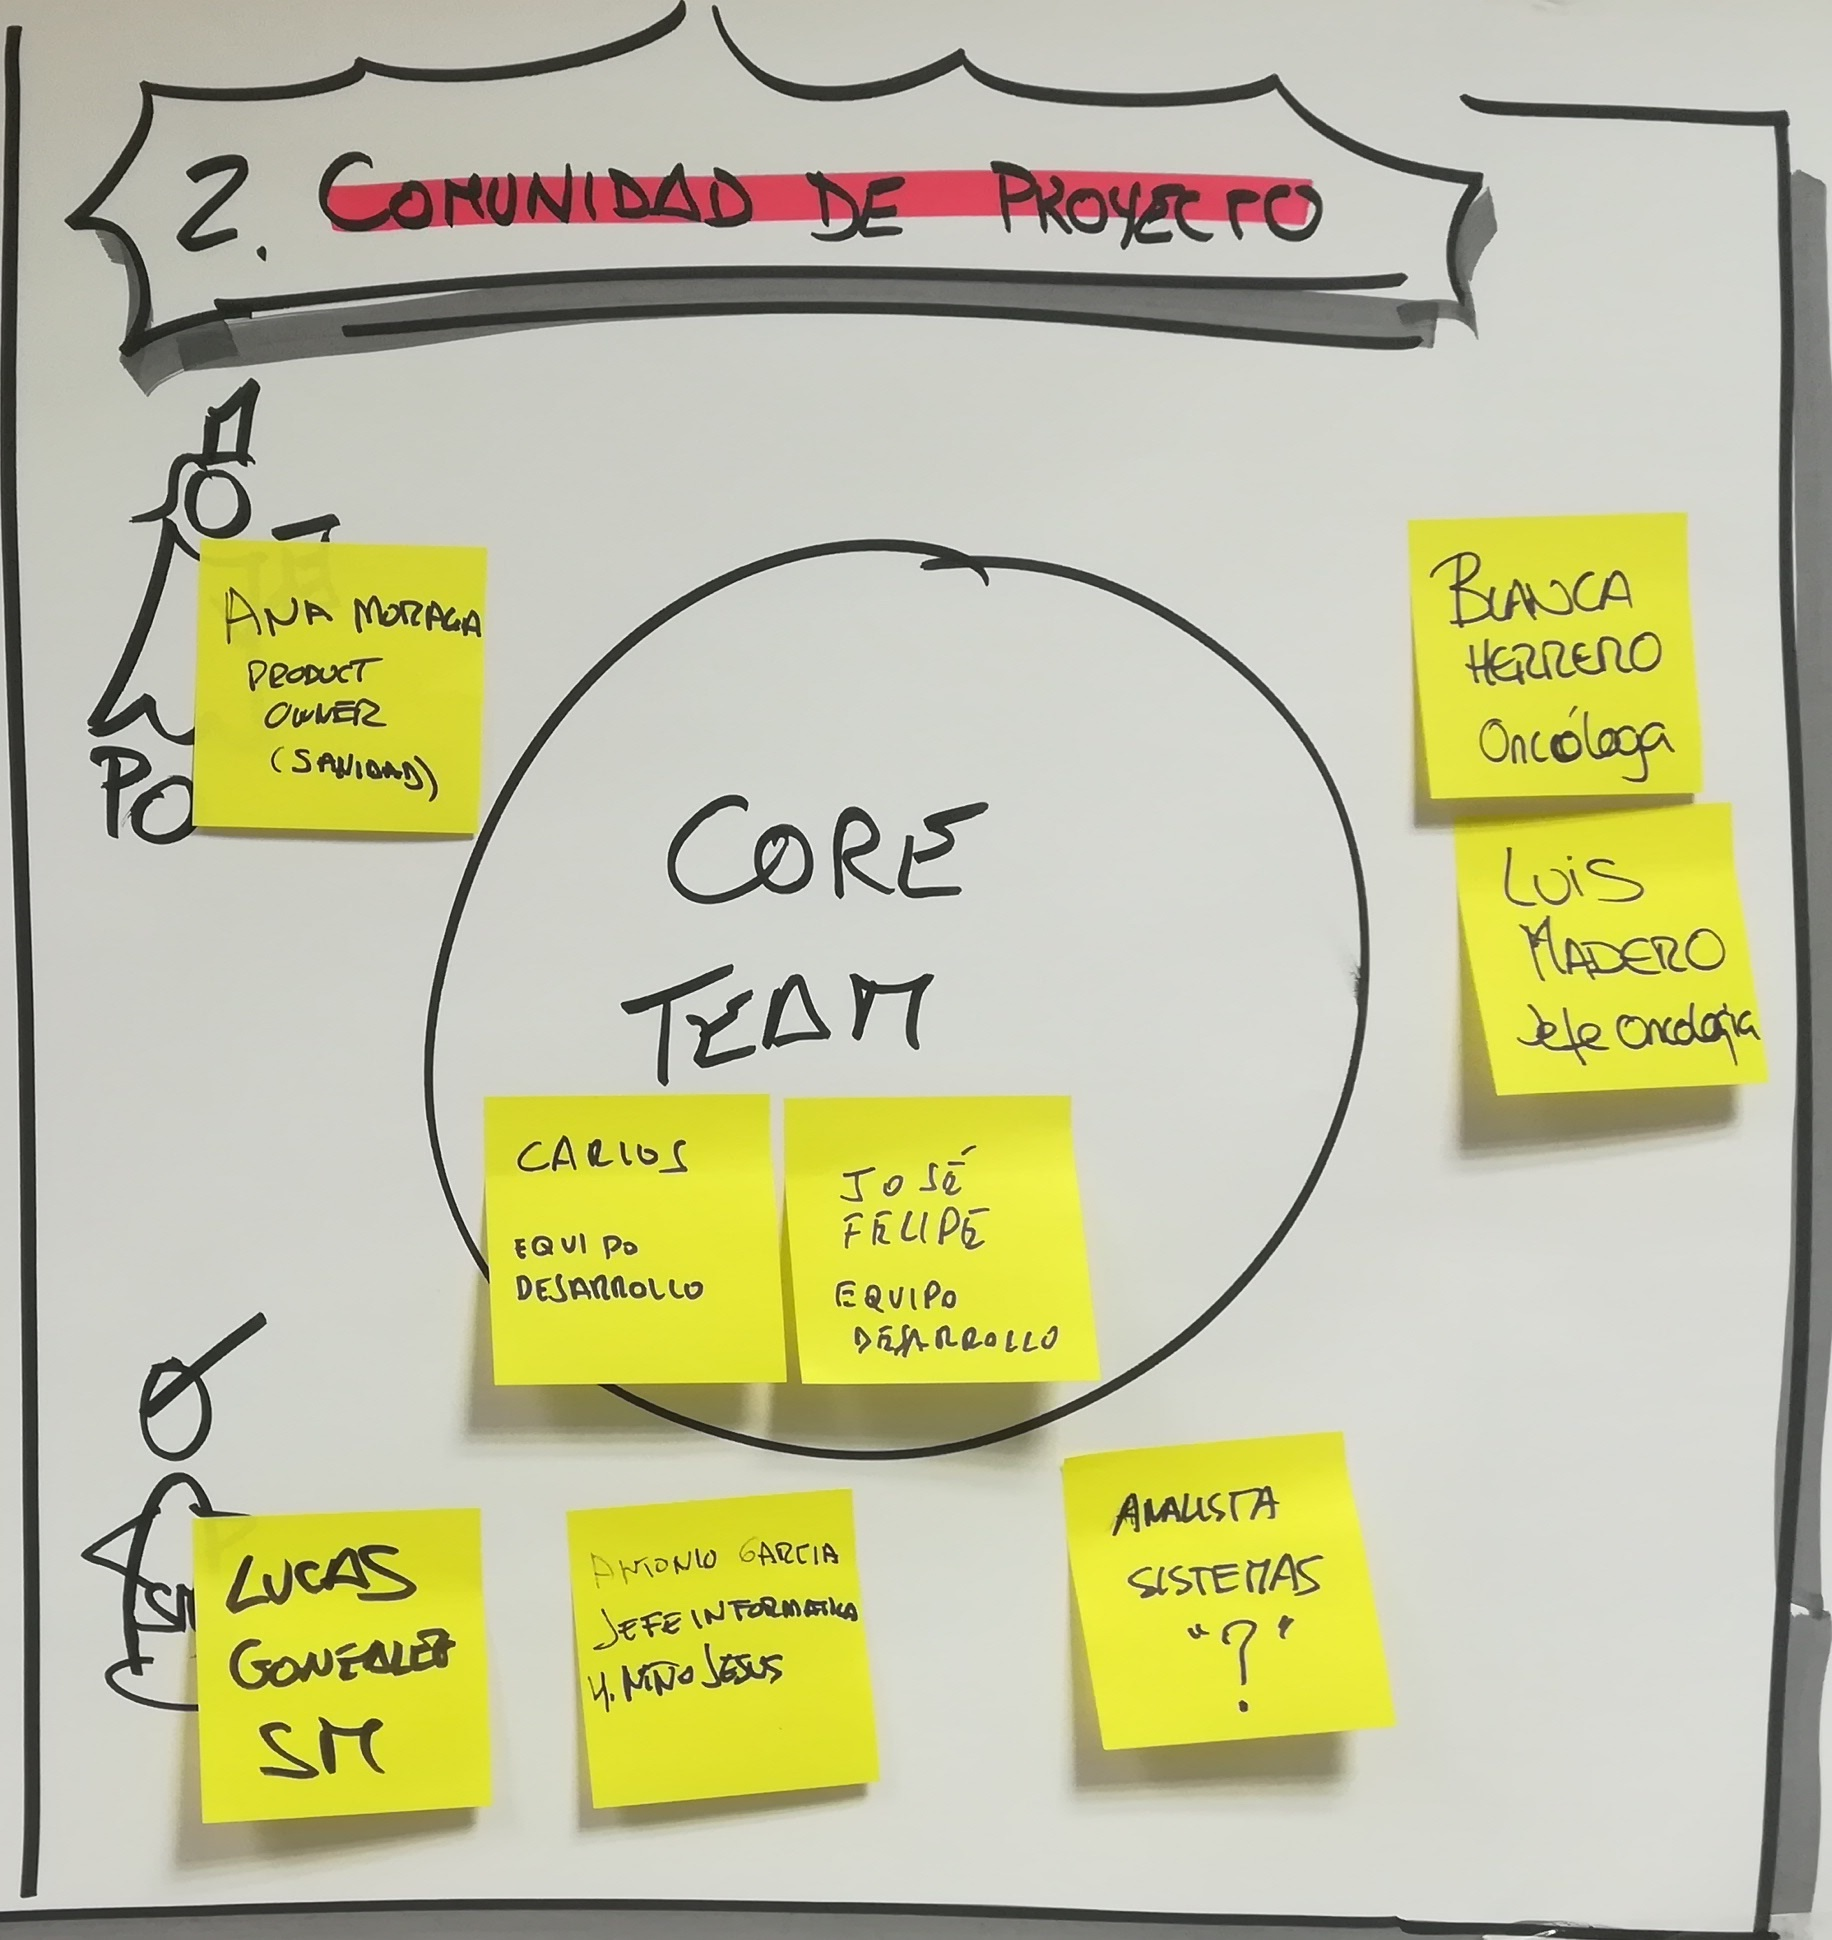
\includegraphics[width=0.50\textwidth]{comunidadDeProyecto}
    \caption{Comunidad de proyecto}
    \label{fig:comunidad}
\end{wrapfigure}
En la figura \ref{fig:comunidad} vemos que la comunidad de proyecto difiere ligeramente de la especificada en el cuadro \ref{tab:comunidad}. Esto se debe a que al comienzo del proyecto, la Dra. Herrero no creía poder dedicar el tiempo necesario al papel de \emph{Product Owner}, pero finalmente trató de organizar su agenda para poder dedicar algunos días ya que ella es la primera interesada en la aplicación, es quien sabe qué necesita de ella y probablemente será la primera usuaria. Por otra parte, el Director de Proyecto de la UCLM y la autora, aparecen en el listado de participantes y no en el panel que se hizo en la \emph{Inception}; la autora se une al proyecto al comienzo del sprint 1, por tanto no se contaba con la participación de ninguno de ellos cuando se realizó esta especificación.

\begin{table}[!h]
\centering
\caption{Detalle de la comunidad de proyecto}
\label{tab:comunidad}
\begin{tabular}{@{}lllll@{}}
\toprule
\rowcolor[HTML]{9B9B9B} 
\multicolumn{5}{c}{\cellcolor[HTML]{9B9B9B}Comunidad de proyecto}                                                                                                                                  \\ \midrule
Stakeholders                & \multicolumn{4}{l}{\begin{tabular}[c]{@{}l@{}}- Carlos Navas (IECISA).\\ - Macario Polo Usaola (Director TFG UCLM).\end{tabular}}                                     \\
\rowcolor[HTML]{EFEFEF} 
Product owner               & \multicolumn{4}{l}{\cellcolor[HTML]{EFEFEF}- Blanca Herrero (Oncóloga HNJ)}                                                                                          \\
Equipo de desarrollo        & \multicolumn{4}{l}{\begin{tabular}[c]{@{}l@{}}- Carlos Romero Martín-Duarte (IECISA).\\ - José Felipe Lozano Gijón (IECISA).\\ - María López %
Carrasco (Autora)\end{tabular}} \\
\rowcolor[HTML]{EFEFEF} 
SCRUM Master                & \multicolumn{4}{l}{\cellcolor[HTML]{EFEFEF}- Lucas González (IECISA).}                                                                                                 \\ \bottomrule
\end{tabular}
\end{table}

\subsection{Restricciones y riesgos.}
\label{subsec:restriccionesRiesgos}


Identificar las restricciones del proyecto es un punto muy importante de la especificación que se realiza en la \emph{Inception}, debido a que una vez identificados los elementos más restrictivos, se les asignará una importancia en la escala de \emph{Trade Offs}. 



También se definen unos riesgos, que son ordenados en una matriz (Figura~\ref{fig:riesgos}). Esto sirve para que el equipo sea consciente del impacto que puede generar si alguno de estos riesgos se llegara a producir. Cuanto más a la derecha se coloca un riesgo mayor impacto puede generar si se produce. Por otro lado, cuanta mayor sea la probabilidad de que suceda, se situará más arriba en la matriz. Se trata de una forma muy visual y fácil de comprender para ordenar los distintos riesgos que pueden afectar al proyecto. Para cada riesgo se definen unas acciones de contingencia, es decir, qué hacer en caso de que ocurra alguno de los riesgos definidos.

\subsubsection{Restricciones}
\label{subsubsec:restricciones}
\begin{wrapfigure}{r}{0.50\textwidth} %this figure will be at the right
    \centering
    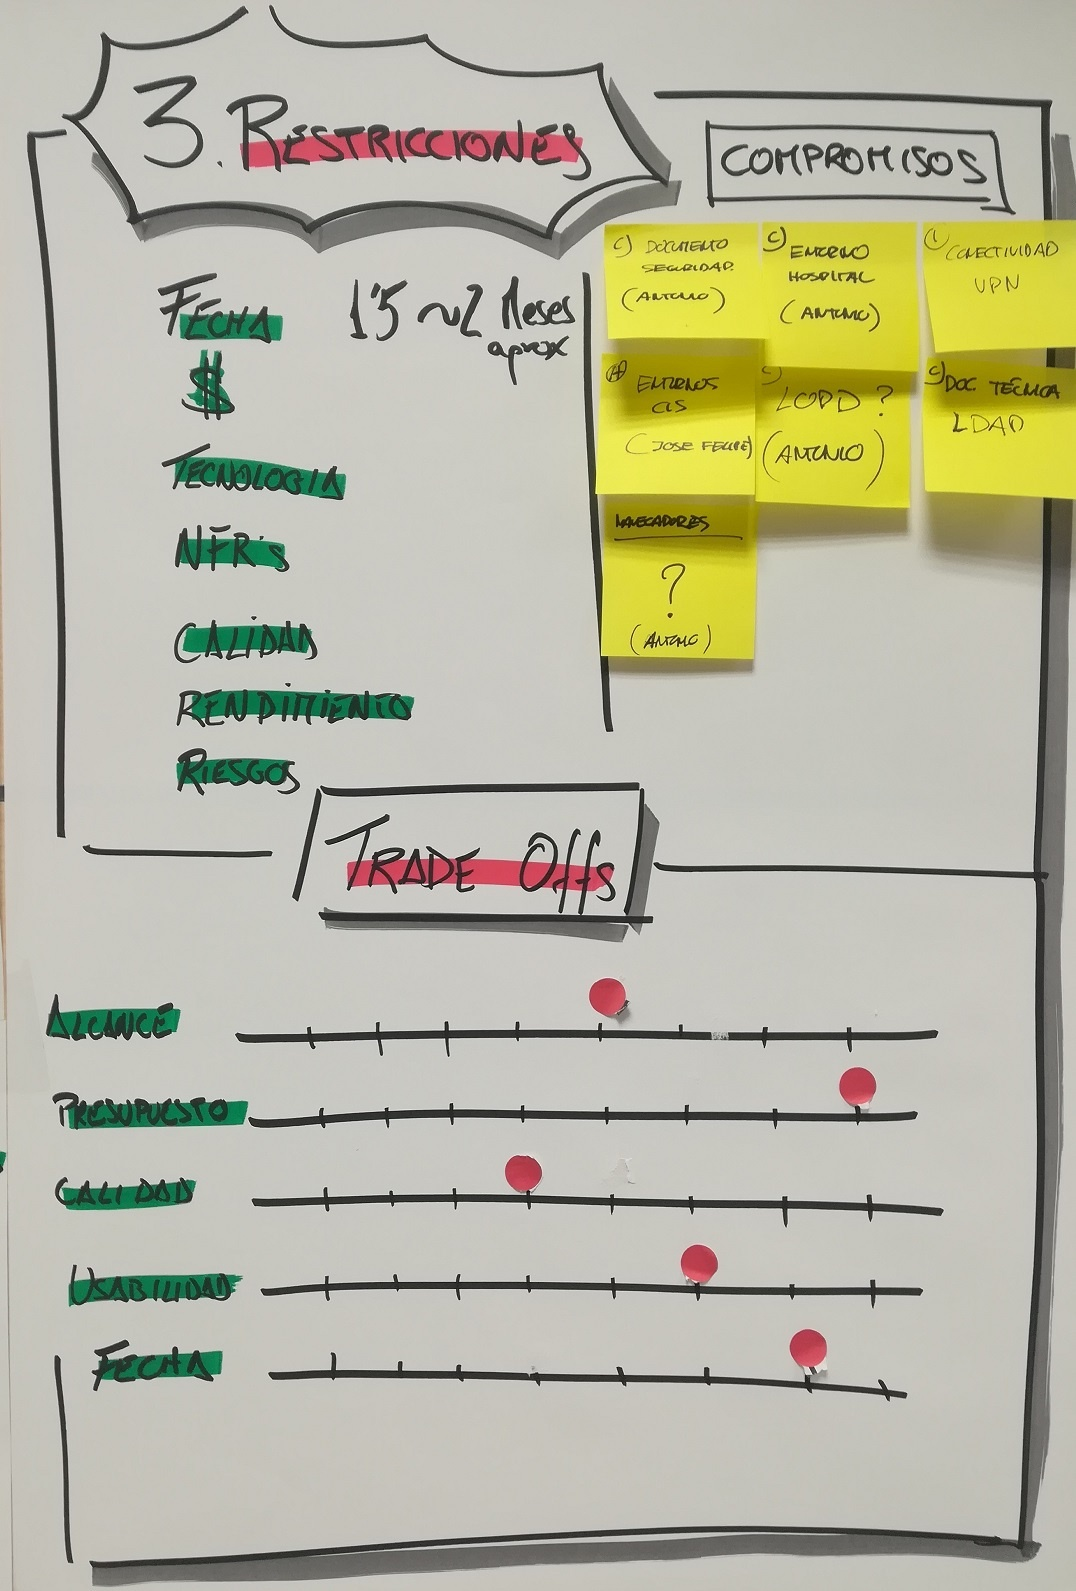
\includegraphics[width=0.50\textwidth]{restricciones}
    \caption{Restricciones y Trade offs}
    \label{fig:restricciones}
\end{wrapfigure}
Como se puede observar en la figura \ref{fig:restricciones}, en la dinámica destinada a esta tarea se deja un espacio lo suficientemente grande en el que se van escribiendo las restricciones que el equipo va identificando. Las restricciones son todos aquellos aspectos que limitan el proyecto. Para ONCOSUP se identificaron:

\begin{itemize}
\item Fecha. La fecha de ONCOSUP es muy restrictiva, pues el cliente quiere que el proyecto esté terminado para el mes de mayo, lo que deja tres meses para su desarrollo.
\item Presupuesto. El presupuesto para el desarrollo es reducido, lo que se traduce en menos personas trabajando en el desarrollo y poca flexibilidad para extender la fecha de entrega.
\item Tecnología. El equipo remitió un documento con las tecnologías a utilizar. Es necesario que el hospital apruebe las tecnologías propuestas por el equipo.
\end{itemize}

\begin{itemize}
\item Requisitos no funcionales (NFR). Es necesario saber qué tipo de restricciones no funcionales habrá por parte del hospital (navegadores, resolución de los equipos, etcétera)
\item Calidad. Se desea que el proyecto tenga la mejor calidad posible, pero será algo que habrá que ir gestionando debido a otras restricciones como la fecha o el presupuesto.
\item Rendimiento. El rendimiento debe ser tan bueno como sea posible, ya que requerirá accesos frecuentes a base de datos.
\item Riesgos. Los riesgos son elementos que el equipo identifica como potenciales situaciones que podrían bloquear el desarrollo.
\end{itemize}

\begin{figure}[!h]
\begin{center}
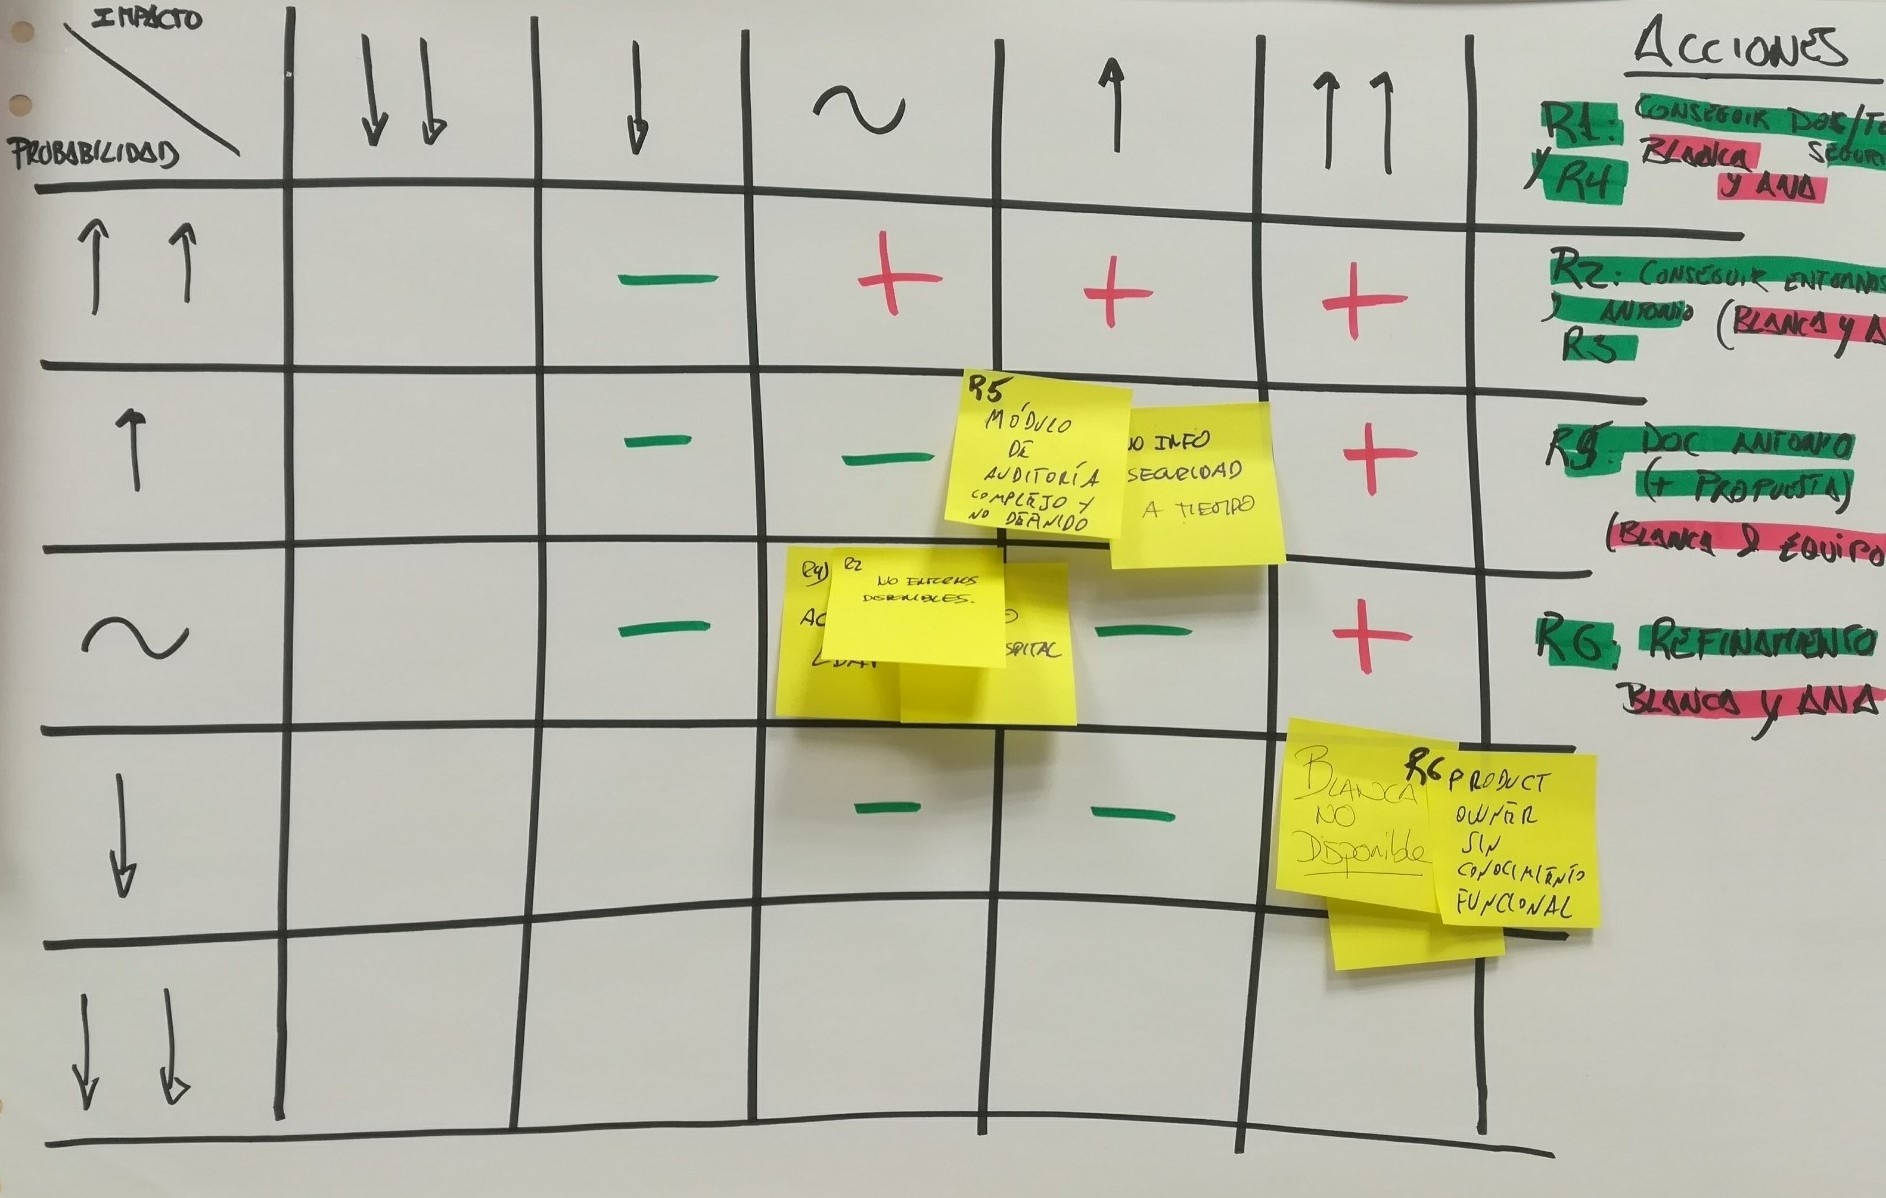
\includegraphics[width=0.9\textwidth]{riesgos}
\caption{Matriz de riesgos}
\label{fig:riesgos}
\end{center}
\end{figure}


\subsubsection{Riesgos}
\label{subsubsec:riesgos}

En lo referente a los riesgos, se identificó la siguiente lista:
\begin{itemize}
\item R1 - No disponer de la información de seguridad a tiempo. Además de los aspectos generales de la Ley Orgánica de Protección de Datos \cite{lopd}, el equipo de desarrollo necesita saber si hay algún tipo de normativa específica a seguir respecto a la seguridad de los datos con los que trata la aplicación.
\item R2 - Entornos no disponibles. Para la realización de pruebas, es necesario saber cuál será el entorno que proporcionará el hospital. Igualmente para el despliegue en producción.
\item R3 - Acceso al hospital. Es necesario poder acceder al entorno del hospital, para ello desde el hospital deben informar sobre cómo acceder a través de VPN.
\item R4 - No se dispone de información sobre el acceso a LDAP \cite{ldap}. En necesario conocer cómo acceder al LDAP, ya que los usuarios de ONCOSUP, serán usuarios del LDAP.
\item R5 - Módulo de Auditoría complejo y no definido. El Módulo de Auditoría es complejo por la naturaleza del proyecto y no está definido qué datos deben guardarse para ser auditados.
\item R6 - Product Owner sin conocimiento funcional. La Dra. Herrero no va a tener mucha disponibilidad durante el proyecto y otra persona debe ejercer de \emph{Product Owner} teniendo menos conocimientos del dominio de la aplicación que la doctora, que es la usuaria final.
\end{itemize}

Una vez identificados los riesgos que hasta el momento pueden afectar al proyecto, el equipo los coloca en la matriz, de manera que de un vistazo se pueda ver cuán importantes es cada uno (Figura~\ref{fig:riesgos}). En el caso de que a lo largo del desarrollo del proyecto se identifiquen nuevos riesgos, se registrarán y se colocarán en la matriz de la misma forma.

\subsubsection{Trade offs}
\label{subsubsec:tradeOffs}

En la parte inferior de la figura \ref{fig:restricciones} vemos cómo se han organizado los \emph{Trade offs} o \emph{palancas}. Para el desarrollo de ONCOSUP lo menos relevante es la calidad, mientras que lo más restrictivo y menos tolerante a cambios será el presupuesto.

A cada elemento se le da un valor de relevancia a la hora de tomar decisiones, colocando los más importantes en la parte derecha y los menos importantes en la izquierda. No se puede asignar el mismo valor dos veces, con lo que se busca que el cliente piense bien qué elementos desea priorizar. Esta escala será la referencia a tomar si durante el desarrollo del proyecto se diera algún conflicto y fuese necesario priorizar un elemento en lugar de otro.


\subsection{Story Map.}
\label{subsec:storyMap}

Teniendo ya claro el objetivo de la aplicación y sus limitaciones, la siguiente fase consiste en definir el \emph{Product Backlog}. 

El equipo trata de definir los \emph{Flujos de negocio}, que son una forma de englobar diferentes historias que estarán relacionadas entre sí en una gran categoría. Cada una de las historias de usuario que se generan es asignada a uno de estos \emph{Flujos de negocio}, permitiendo al equipo tener una visión más organizada de las diferentes partes que compondrán la aplicación. 

\begin{wrapfigure}{r}{0.35\textwidth} %this figure will be at the right
    \centering
    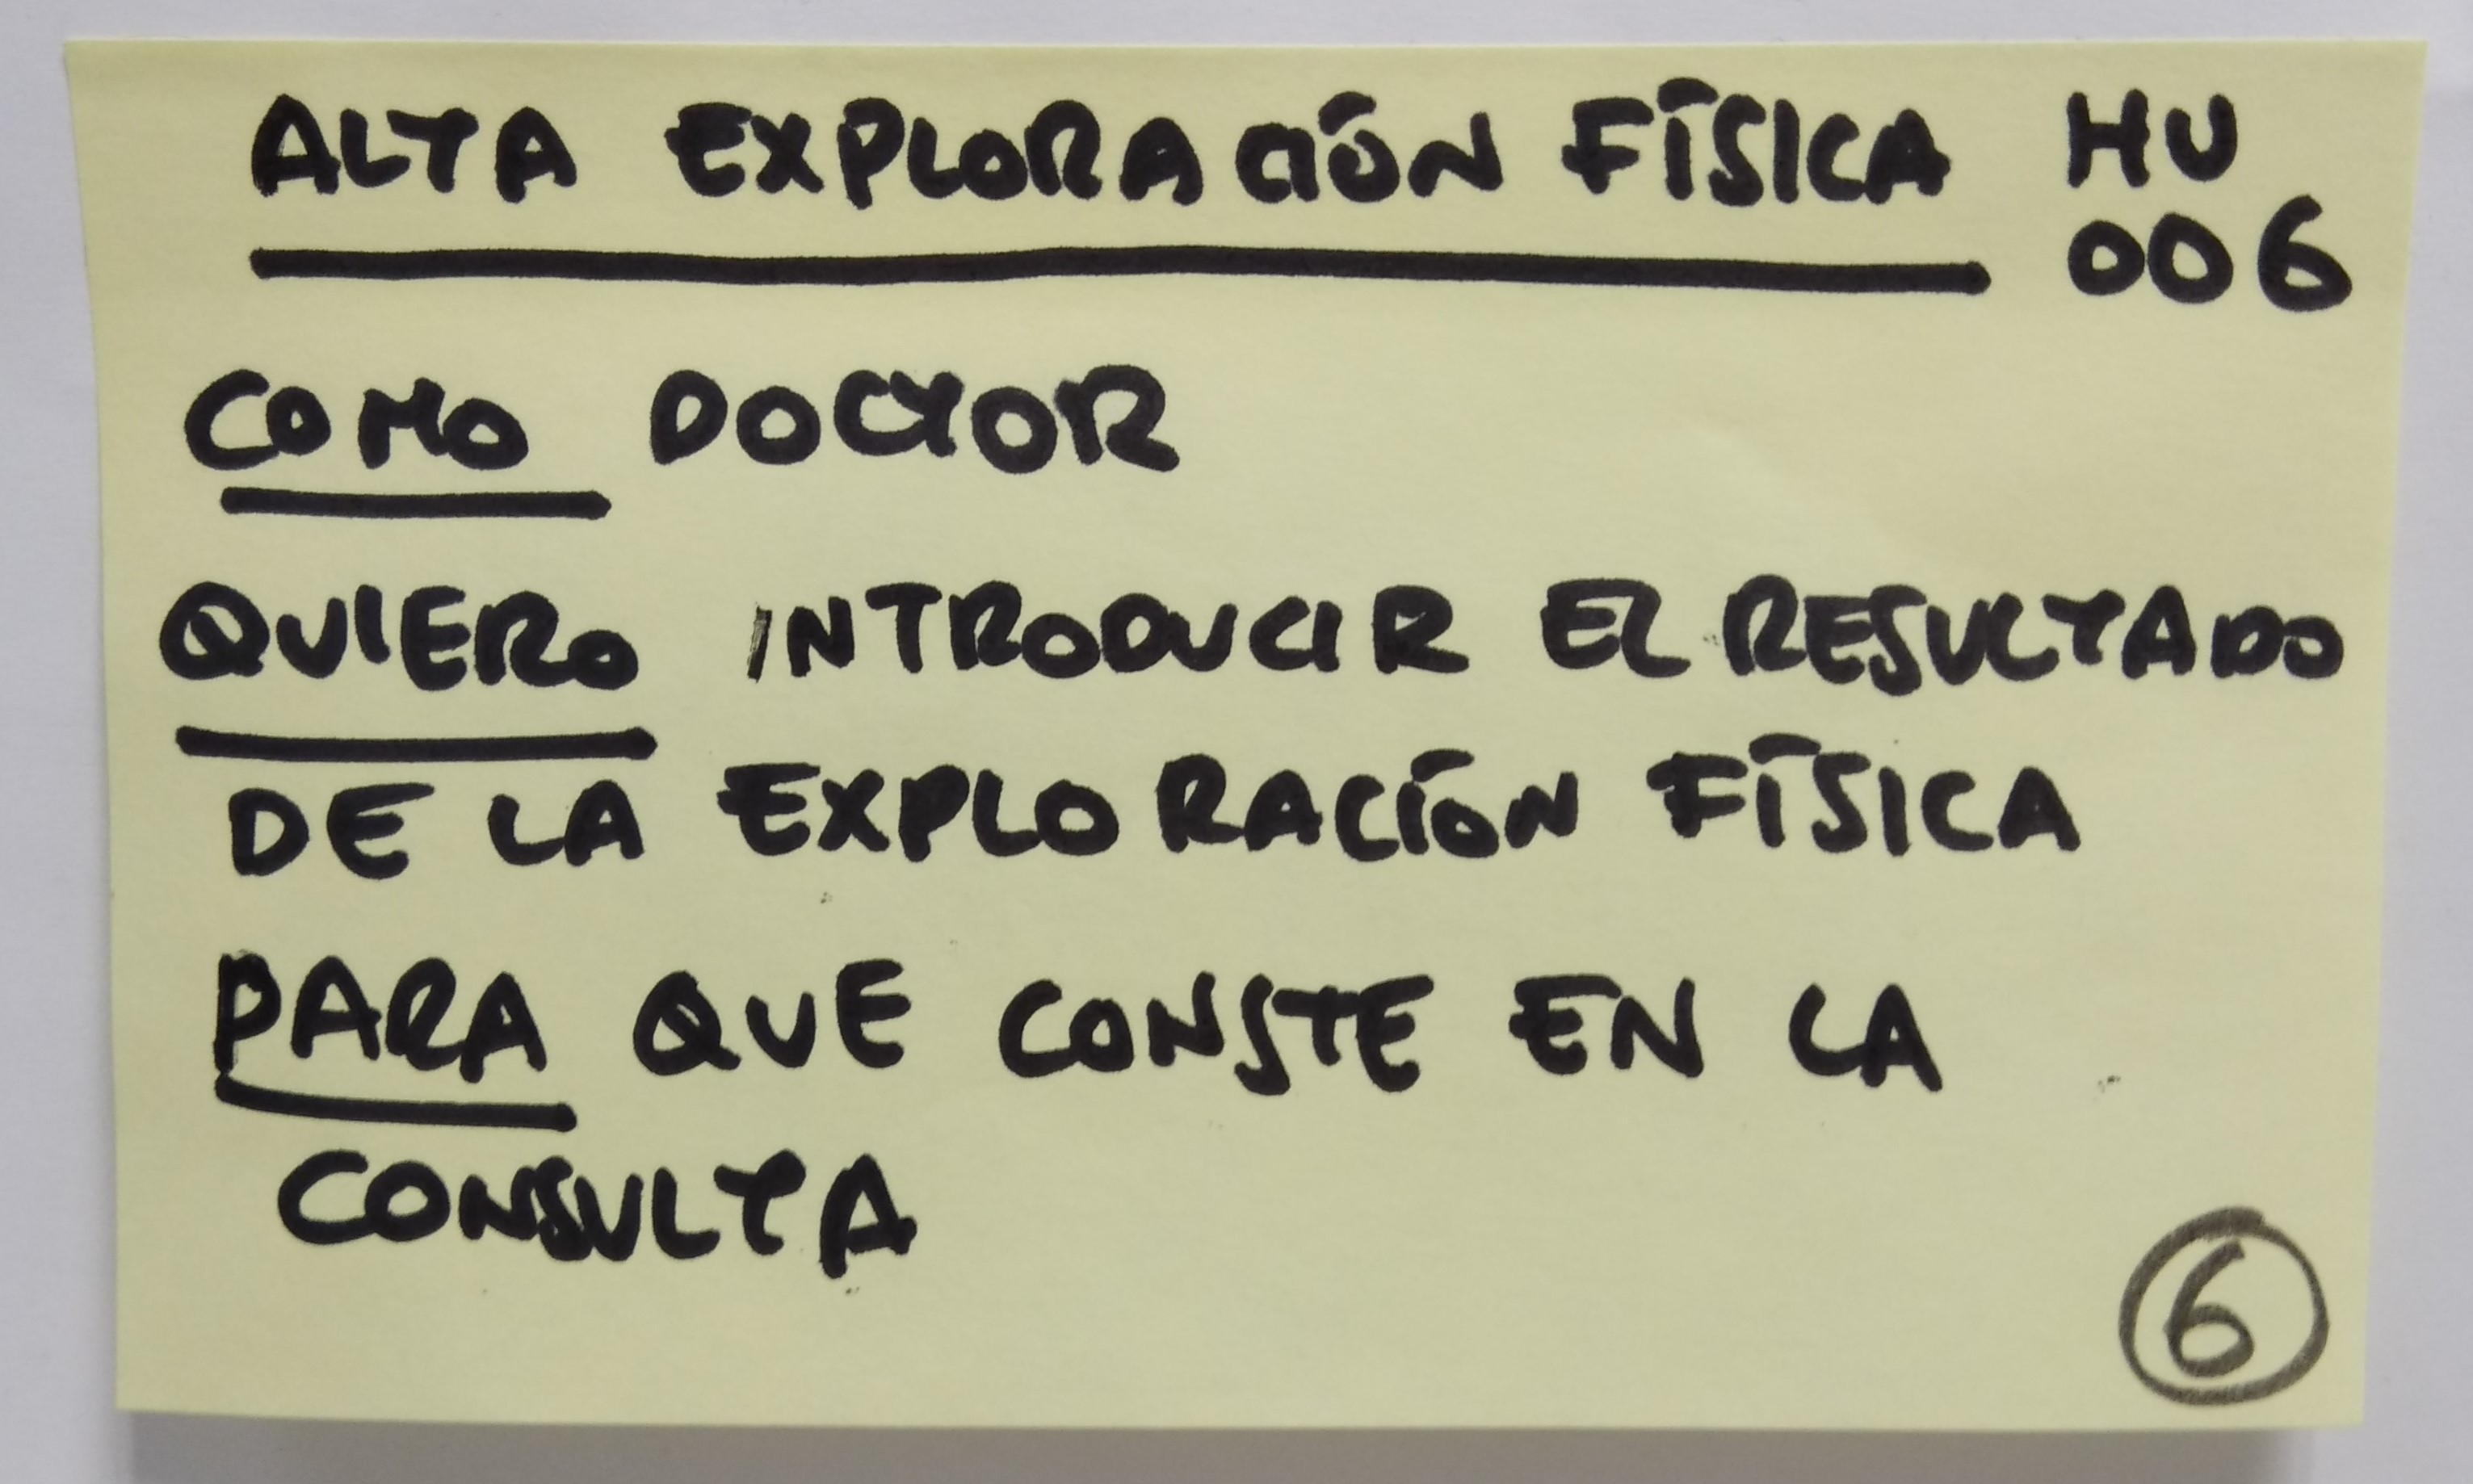
\includegraphics[width=0.35\textwidth]{historia_usuario}
    \caption{Ejemplo de una Historia de Usuario}
    \label{fig:historia}
\end{wrapfigure}
El \emph{Scrum Master} ayuda al \emph{Product Owner} y al equipo de desarrollo a definir las historias de usuario dándoles unas directrices sobre su extensión, estructura, los criterios de aceptación, etcétera. Así se escriben estas historias en pósits (Figura~\ref{fig:historia}), que luego se colocan en el panel del \emph{Story Map}, dónde se ponen según la priorización que el \emph{Product Owner} considera.

Además de las 26 historias de usuario que se han definido en esta etapa, se seleccionan las historias que compondrán el \emph{Producto Mínimo Viable} (MVP), que en este caso son las que están por encima de la línea roja (Figura~\ref{fig:backlog}). Cuando esas historias hayan sido completadas, se obtendrá una versión mínima que aportará valor al cliente, que en este caso se corresponde con la \emph{épica} de \emph{Estudio preconsulta} y \emph{Administración} casi en su totalidad. El motivo de haber seleccionado estas historias como MVP es que cuando estén completadas, permitirán a la doctora comenzar a introducir prácticamente todos los datos que necesita antes de pasar las consultas, de manera que podría ir preparando la base de datos con la información que considere.
\\
\begin{figure}[!h]
\begin{center}
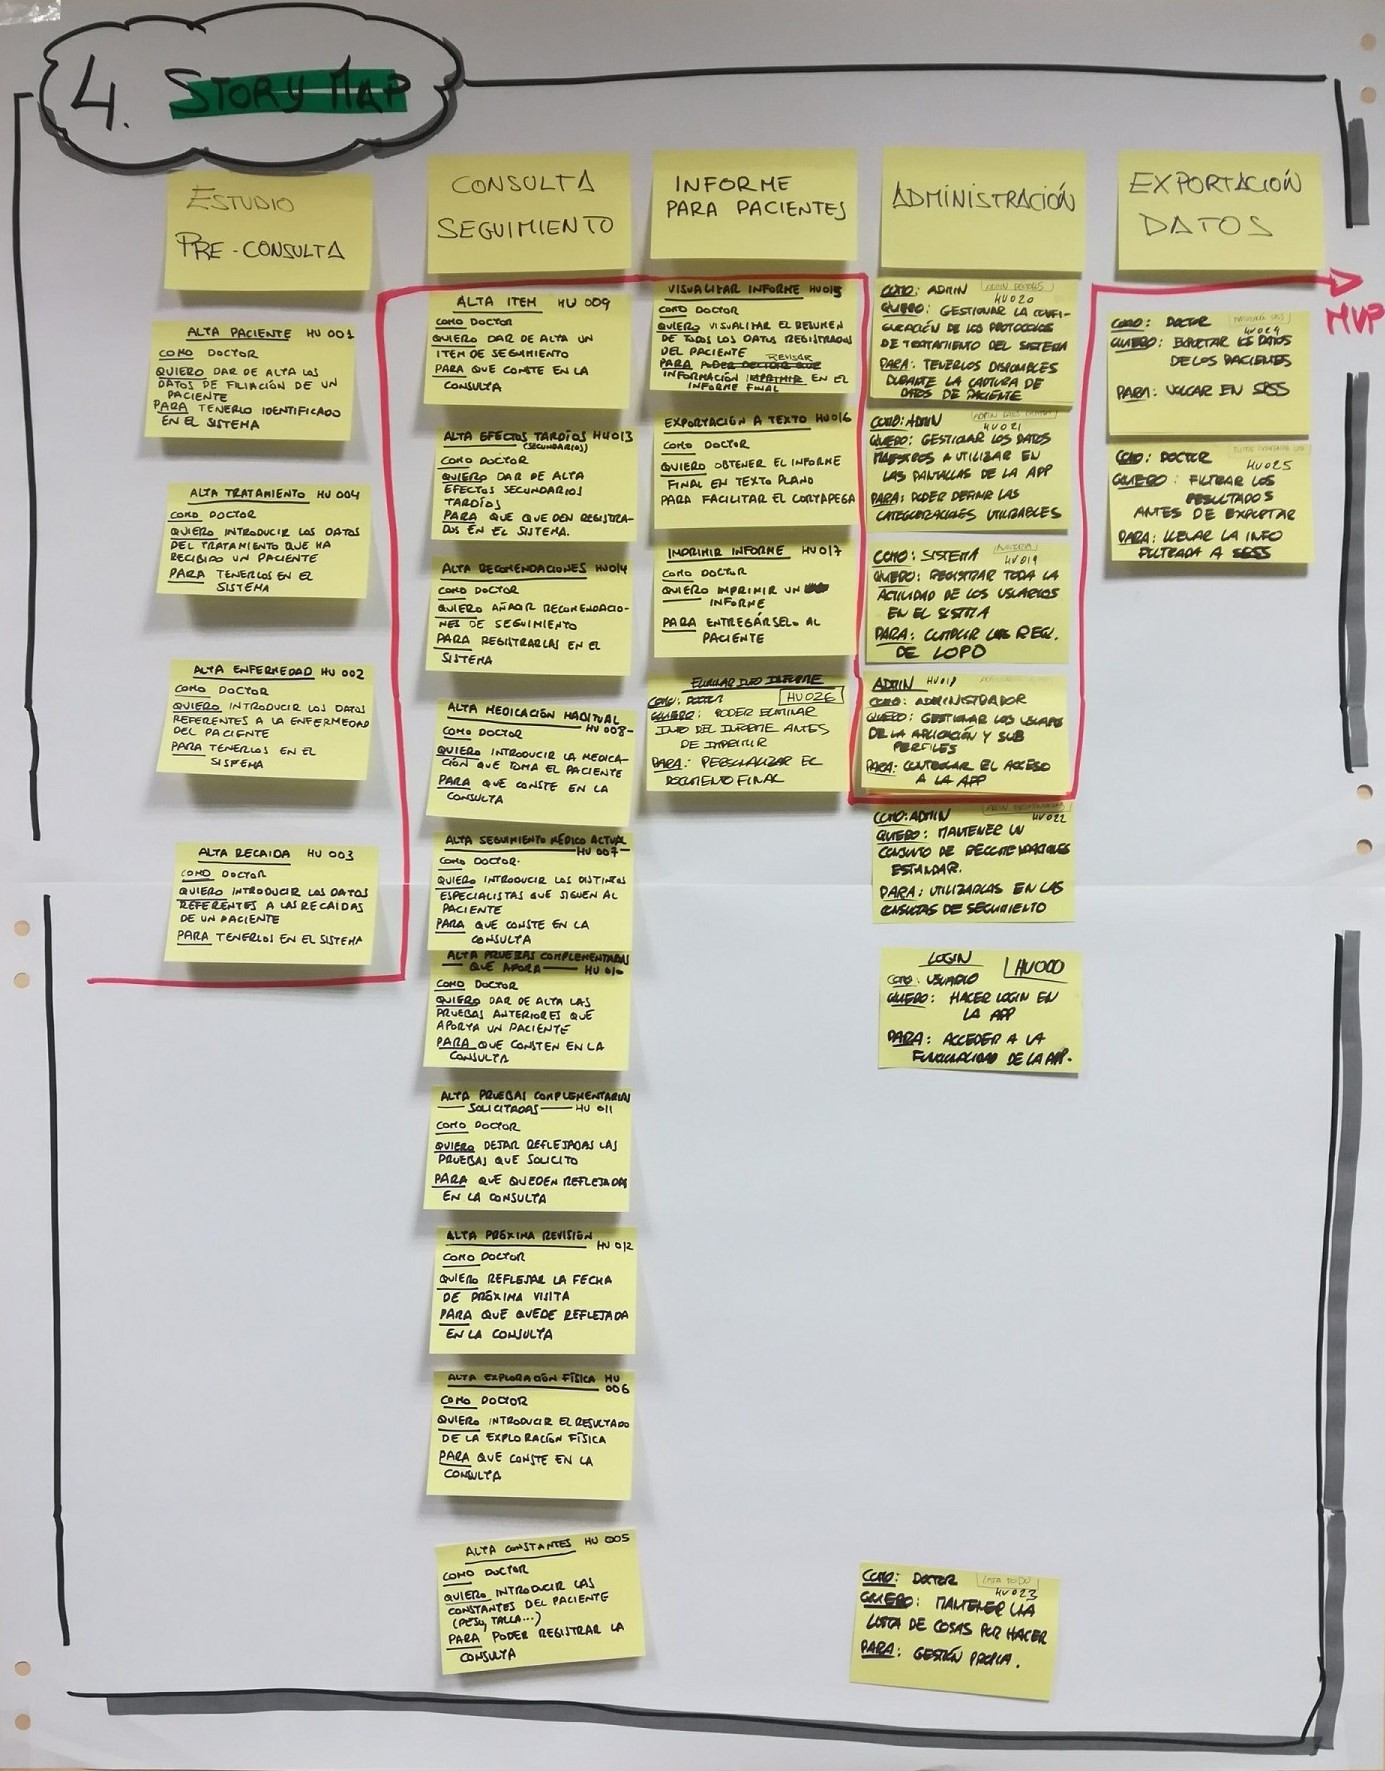
\includegraphics[width=0.95\textwidth]{product_backlog}
\caption{Product Backlog}
\label{fig:backlog}
\end{center}
\end{figure}

\subsection{Volcado en JIRA y Confluence.}
\label{subsec:volcado}

Toda la información obtenida en estos talleres se registra para permitir al equipo gestionar todo el proceso de desarrollo del proyecto. Así, al acabar la \emph{Inception}, el equipo registra todo en \emph{Confluence} para documentar el desarrollo del proyecto, y en \emph{JIRA} para su gestión del desarrollo.

\begin{wrapfigure}{l}{0.30\textwidth} %this figure will be at the right
    \centering
    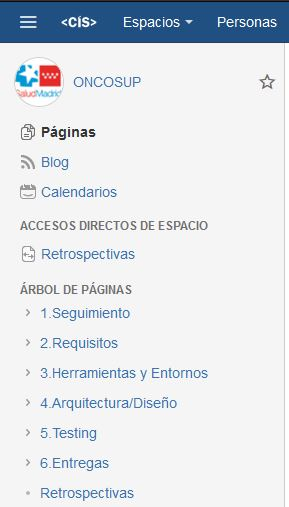
\includegraphics[width=0.30\textwidth]{indiceConfluence}
    \caption{Indice de la documentación del proyecto}
    \label{fig:indiceConfluence}
\end{wrapfigure}

\emph{Confluence} es una \emph{wiki} abierta a todo el equipo que organiza la información de forma arborescente (Figura~\ref{fig:indiceConfluence}).

A la autora le ha parecido de especial interés la sección "Lecciones aprendidas", en la que los miembros del equipo anotan diferentes problemas que han surgido durante el proyecto y cómo solucionarlos, permitiendo encontrar solución rápida a problemas recurrentes o que no son fáciles de resolver. Además, los usuarios reciben notificaciones cuando se crea una nueva entrada en un espacio que siguen en \emph{Confluence}, facilitando que todos los miembros del equipo estén al tanto de las actualizaciones que se hagan.

Al inicio del proyecto y haciendo uso de una gran cantidad de funcionalidades que \emph{JIRA} pone a disposición de sus usuarios se registran todos los artefactos que se han generado durante el desarrollo de la \emph{Inception}. Es posible registrar las historias de usuario, los riesgos del proyecto, los compromisos, tareas y subtareas relacionadas con el proyecto, lo que ayuda a la gestión de este, permitiendo tener toda la información importante en un mismo espacio. 

Además, como tanto \emph{JIRA} como \emph{Confluence} y \emph{BitBucket} son todas herramientas de \emph{Atlassian}, es posible, enlazar referencias de diferentes elementos creados en una herramienta a otro elemento creado en otra distinta. Por ejemplo, en el espacio de \emph{Confluence} de ONCOSUP, en el apartado de compromisos, hay enlaces a los elementos creados en \emph{JIRA}, dónde están especificados, o al subir código al repositorio (\emph{commit}) podemos referenciar la tarea con la que corresponde la codificación que se va a subir al repositorio.

Por otra parte, en la sección \ref{subsubsec:restricciones} se hablaba de la matriz de riesgos, esta matriz no es algo que se hace en papel durante la \emph{Inception} sin más, sino que la propia herramienta \emph{JIRA} (ver Figura~\ref{fig:matrizRiesgos}), con la información que se aporta al registrar un riesgo, genera esa matriz. Esta matriz se va actualizando según los riesgos se van resolviendo o aparecen nuevos, siendo lo ideal que al final del proyecto la matriz esté vacía. La matriz de riesgos se puede ver tanto desde \emph{JIRA} como desde el espacio en \emph{Confluence}, ya que ambas herramientas se sincronizan, en este caso la matriz que se muestra es la que se puede ver desde \emph{Confluence}. También se aprecia que la matriz que muestra la figura \ref{fig:matrizRiesgos} se corresponde con la figura \ref{fig:riesgos} de la sección \ref{subsubsec:restricciones}.
\\
\begin{figure}[!h]
\begin{center}
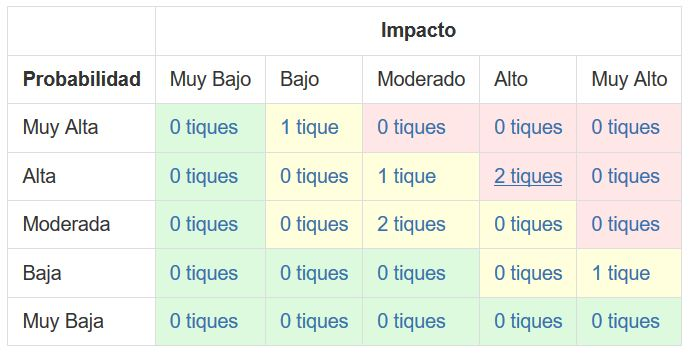
\includegraphics[width=1\textwidth]{matrizRiesgos}
\caption{Matriz de riesgos en Confluence}
\label{fig:matrizRiesgos}
\end{center}
\end{figure}
\\
\\
\\
\\
\\
\section{Incorporación a IECISA}
\label{sec:incorporacion}

La autora se incorpora a la actividad de la empresa el día 5 de febrero de 2018, coincidiendo precisamente con el comienzo del primer sprint. 

Justo la primera actividad que se realizó al incorporarse la autora, y sin apenas tiempo para aclaraciones, fue el \emph{Sprint planning} del Sprint 1 que se detalla en la sección \ref{sec:sprint1}. Tras este primer contacto con el proyecto se informó a la autora de todo lo ocurrido en el sprint 0 (ver sección~\ref{sec:sprint0}) y en la \emph{Inception} (ver sección~\ref{sec:inception}), además de proporcionársele toda la documentación registrada en \emph{Confluence} y la información del proyecto en \emph{JIRA} con el fin de que durante los primeros días, y hasta que llegasen los equipos de trabajo, pudiera empaparse tanto como fuese posible sobre el proyecto.

Durante los primeros días, tanto a la autora como al resto de alumnos de FORTE en la empresa, se les dio una breve formación sobre SCRUM. La gran mayoría de los proyectos en IECISA usan este marco de trabajo para la gestión de sus proyectos, por lo que consideran muy importante conocerlo desde el primer día. Además, se animó a todos los FORTE a ``trastear'' con las herramientas (\emph{JIRA} y \emph{Confluence} principalmente) durante estos primeros dias de aclimatación a la empresa.

De los artefactos producidos en la \emph{Inception} y elementos que componen el proyecto, resultan de especial interés para la autora los que se describen en el listado a continuación:
\\
\\
\\
\begin{itemize}
\item El equipo - Conocer a Carlos y José Felipe como compañeros de trabajo y al resto de la comunidad del proyecto es de especial relevancia en la incorporación al proyecto.
\item Historias de Usuario - A la autora le habría resultado interesante poder asistir a la \emph{Inception} y haber vivido cómo se generan estos artefactos y cómo todo el equipo trabaja para definir cada funcionalidad de la aplicación.
\item MVP - Es también de interés cómo se decide el número mínimo de historias que aporta valor al cliente.
\item Tecnologías - Por el poco presupuesto y el tiempo reducido se utiliza JHipster para la generación del esqueleto o arquitectura de la aplicación. Esta herramienta utiliza muchas otras para esta generación como, por ejemplo, Angular5, Spring Boot, Apache Tomcat, etcétera.
\end{itemize}

Después de ponerse al día con el proyecto y las herramientas que se utilizan en la empresa, la autora dedicó tiempo al estudio y aprendizaje de las diferentes tecnologías que se usan en el proyecto. En su front-end es dónde se incorpora la autora. La aplicación utiliza un patrón de diseño MVC que, pese a ser contenido que se estudia durante el desarrollo de la carrera, se trata de una arquitectura de aplicación con el que la autora apenas ha tenido experiencia; de esta forma, otra de las actividades que la autora hizo durante los primeros días, esta vez ya de forma individual, fue refrescar conocimientos y afianzar algunos nuevos respecto al MVC.

JHipster, herramienta principal que genera código para distintas herramientas. De todas las que usa quizá las más importantes y de las que menos conocimientos tiene la autora son Angular5 y Spring Boot. Spring Boot se trata de la herramienta principal que usa JHipster para generar la arquitectura de nuestra aplicación, esta herramienta se utiliza de forma simple, indicándole las características de nuestro proyecto nos generará la estructura básica de la aplicación. Además, JHipster se vale de Angular5 para generar el front-end de nuestra aplicación. De la misma forma que con el MVC, se dedicó parte de estos días al aprendizaje de Angular5 como framework de desarrollo front-end y el lenguaje \emph{TypeScript} muy similar a \emph{JavaScript}.

En figura \ref{fig:angularMVC}, a continuación, se puede ver cómo es la arquitectura de la aplicación. Vemos la arquitectura habitual de un patrón MVC, siendo el cliente la vista, y estando en el servidor el controlador y el modelo que se comunica con la base de datos. Todos los elementos del servidor usan el framework de Spring para comunicarse entre ellos.

Se puede apreciar que Angular 5, nos genera un cliente basado en el patrón MVC también.

\begin{figure}[!h]
\begin{center}
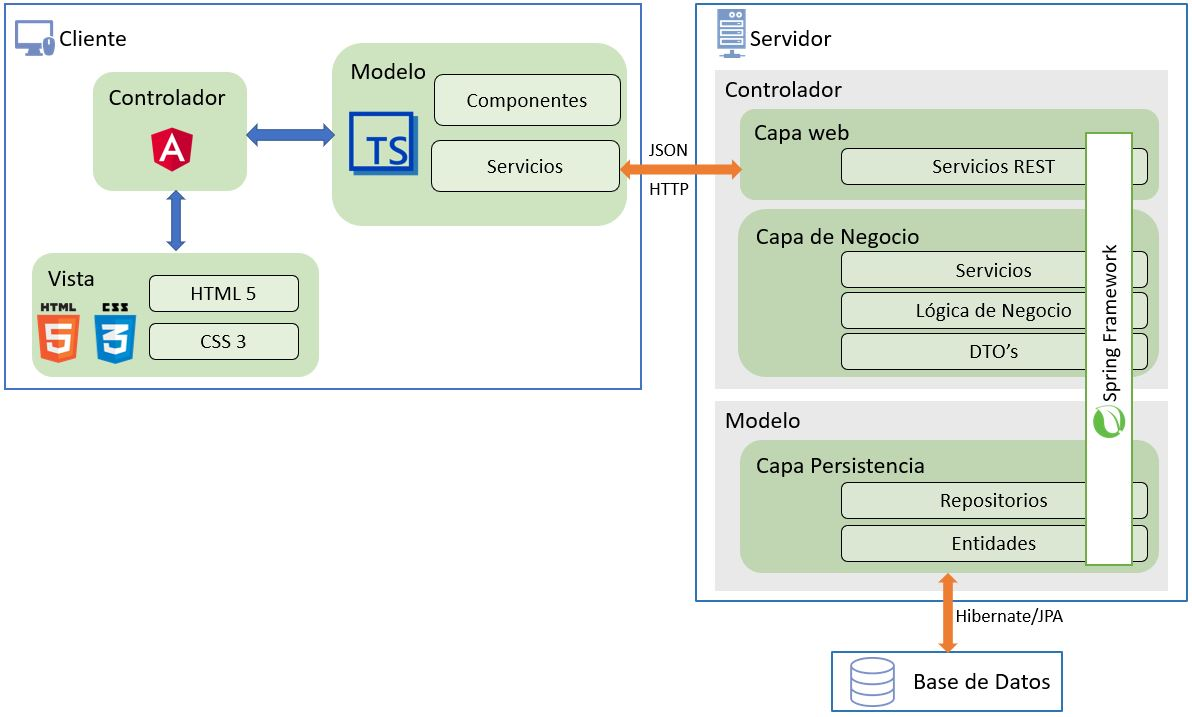
\includegraphics[width=1\textwidth]{AngularMVC}
\caption{Arquitectura de la aplicación}
\label{fig:angularMVC}
\end{center}
\end{figure}

\section{Sprint 0}
\label{sec:sprint0}

El fin de este sprint inicial es decidir qué herramientas se van a utilizar para el desarrollo del proyecto. Para ello, se proponen diferentes opciones y se realizan distintas pruebas. En función de los resultados obtenidos se toma la decisión de cuál es la más adecuada. 

El presupuesto de ONCOSUP es reducido, lo que se traduce en un equipo de desarrollo pequeño y un tiempo limitado para completar el proyecto. El equipo al que se une la autora es el autodenominado ``Equipo Negro'', compuesto únicamente por dos miembros: Carlos Romero Martín-Duarte y José Felipe Lozano Gijón. 

Debido a las limitaciones del proyecto el equipo decidió probar una herramienta relativamente nueva: JHipster. Se trata de una plataforma de desarrollo para generar, desarrollar y desplegar aplicaciones web con Spring Boot y Angular5. Se tomó la decisión de probar JHipster con la idea de poder generar el esqueleto de la aplicación que se quería desarrollar, para después moldearla según las necesidades del proyecto, y así ser capaces de cubrir el alcance del proyecto a pesar de ser únicamente dos miembros en el equipo.

Como resultado de las pruebas de este sprint, se confirma que JHipster es la herramienta que se usará para el desarrollo. Si bien la herramienta debería facilitar al equipo conseguir desarrollar la aplicación en menos tiempo del que es habitual para aplicaciones de este tipo, se tiene en cuenta que será necesario que los miembros de equipo de desarrollo aprendan Angular5, framework que hasta el momento ninguno había usado, lo que puede ralentizar el desarrollo al inicio del mismo, pero se espera que el equipo vaya adquiriendo el conocimiento suficiente como para acelerar el ritmo y ser capaces de llegar a cumplir con el proyecto en la fecha acordada. También se asumen ciertas restricciones en favor de conseguir tener el proyecto dentro del tiempo y presupuesto acordado, por ejemplo, la personalización de estilos será limitada, JHipster ya crea una aplicación relativamente maquetada y responsiva, que se modifica en la menor medida posible; hay decisiones de diseño que es necesario descartar adaptándonos a lo que JHipster nos genera, esto supone cambiar la idea de cómo será la navegación (que en un principio iba a basarse en pestañas) requiriendo aprender cómo JHipster, junto con Angular5, gestiona el acceso, creación y edición de los diferentes elementos que componen la aplicación y ser capaces de modificarlo para que la aplicación se comporte como se desea.

En este sprint también se decide qué software se usa para la base de datos. Inicialmente se pretendía usar MySQL, pero sería necesario pagar una licencia si nuestra aplicación no es \emph{open source} \cite{mysqlpago}; se decide entonces, usar MariaDB que nos ofrece más opciones de almacenamiento que MySQL y operaciones más rápidas \cite{mdbfeatures}.

SCRUM no define dentro de su marco de trabajo un sprint 0, pero fomenta el agilismo\footnote{Aunque la traducción correcta de \emph{agile} sería agilidad, agilismo es la traducción que se usa en desarrollo de software para denominar esta corriente. https://es.wikipedia.org/wiki/Agilismo}, lo que nos permite tomar decisiones sobre cómo afrontar ciertos riesgos en función de las necesidades del proyecto. Es por esto que se ha realizado este primer sprint, que, aunque no forma parte del desarrollo del mismo, sí que será muy útil de cara a que el equipo tome la mejor decisión según las necesidades del producto.


\section{Sprint 1}
\label{sec:sprint1}

El primer sprint de ONCOSUP comienza el día 5 de febrero, como ya se ha mencionado al inicio de la sección \ref{sec:incorporacion}. En el capítulo \ref{chap:metodo} se habla de que la duración de los sprints es de dos semanas, por tanto este primer sprint finaliza el día 16 de febrero.

La primera actividad que se realiza al comenzar cualquier sprint es el \emph{Sprint Planning}, al que la autora se une inmediatamente el día de la incorporación a IECISA. 

\subsection{Sprint Planning}
\label{subsec:S1-SP}
Unos minutos antes de comenzar el \emph{Sprint Planning}, los miembros del equipo de desarrollo y el \emph{Scrum Master} le explicaron a la autora de qué trataba el proyecto para que pudiera comprender lo que se iba a hacer en esta reunión. Una vez aclarado lo que se iba a hacer, el equipo se conecta a través de videoconferencia con la \emph{Product Owner}, se abre \emph{JIRA} para ver las historias del proyecto y la pantalla se comparte con la \emph{Product Owner} y se proyecta para que todos los participantes puedan ver la herramienta.

Hay que decidir qué historias serán las que se abordarán en este sprint, en la \emph{Inception} ya se habían organizado las historias por orden de prioridad, así que ahora, tras haber hecho una estimación del tiempo que llevará completar cada historia, se seleccionan tantas historias como el equipo cree que será capaz de completar de las de mayor prioridad. Además de esta selección de historias se hace un \emph{refinamiento}, que consiste en revisar la especificación inicial de la historia que se introdujo al registrarla en \emph{JIRA}, y que el \emph{Product Owner} aclare, cambie o concrete más las características de ésta o las posibles dudas que el equipo de desarrollo pueda tener a la hora de abordar la historia. Tras unas horas de reunión, finalmente se planificaron y refinaron las siguientes historias para el Sprint 1 (ver cuadro~\ref{historiasSprint1}).

\begin{table}[!h]
\centering
\caption{Historias planeadas Sprint 1}
\label{historiasSprint1}
\begin{tabular}{llr}
\rowcolor[HTML]{C0C0C0} 
\multicolumn{1}{c}{\cellcolor[HTML]{C0C0C0}Identificador} & \multicolumn{1}{c}{\cellcolor[HTML]{C0C0C0}Resumen} & \multicolumn{1}{c}{\cellcolor[HTML]{C0C0C0}Puntos historia} \\
HU001                                                     & Alta Paciente                                      & 11                                                          \\
\rowcolor[HTML]{EFEFEF} 
HU002                                                     & Alta Enfermedad                                    & 6                                                           \\
HU020A                                                   & Administrar Protocolos                              & 12                                                          \\
\rowcolor[HTML]{EFEFEF} 
HU020B                                                   & Administrar Fármacos                                & 8                                                          
\end{tabular}
\end{table}

\begin{itemize}
\item HU001 -Alta Paciente. El objetivo de esta historia es poder dar de alta a un paciente en la base de datos. Es necesario introducir valores como su nombre, nacionalidad u hospital en el que se le trató. Una vez creado un paciente debe ser posible asociarle un diagnóstico.
\item HU002 - Alta Enfermedad. Se necesita poder dar de alta enfermedades, en concreto los diagnósticos. Un diagnóstico tiene campos como fecha, patología, localización, etcétera. Estos diagnósticos deben poder ser enlazados a pacientes existentes en la base de datos.
\item HU020A - Administrar Protocolos. Es necesario poder crear protocolos, es decir, poder definir cómo se trata la dolencia de un paciente.
\item HU020B - Administrar Fármacos. Se desea poder dar de alta diferentes fármacos para poder asignarlos en el futuro a la hora de crear tratamientos.
\end{itemize}

A la hora de refinar las historias se refleja lo especificado en la reunión en cada una de las historias en \emph{JIRA}. La figura \ref{fig:HU002} muestra un recorte de \emph{JIRA} en dónde se puede ver cómo queda reflejada toda la información referente a una historia de usuario; bajo la descripción de la historia se concretan los criterios de aceptación de forma más o menos específica, dependiendo habitualmente, de la complejidad de la historia. Además, para cada historia de usuario se crean unas sub-tareas que también quedan reflejadas en \emph{JIRA}. Estas subtareas sirven para facilitar el trabajo dividiéndolo en otras más sencillas, y para además llevar un mejor seguimiento del avance del proyecto; si no hubiera sub-tareas, una historia no se podría cerrar hasta haberla completado en su totalidad, en cambio con esta división, se pueden cerrar sub-tareas y de esta forma poder visualizar cuánto queda por completar de cada historia de usuario.

\begin{figure}[!h]
\begin{center}
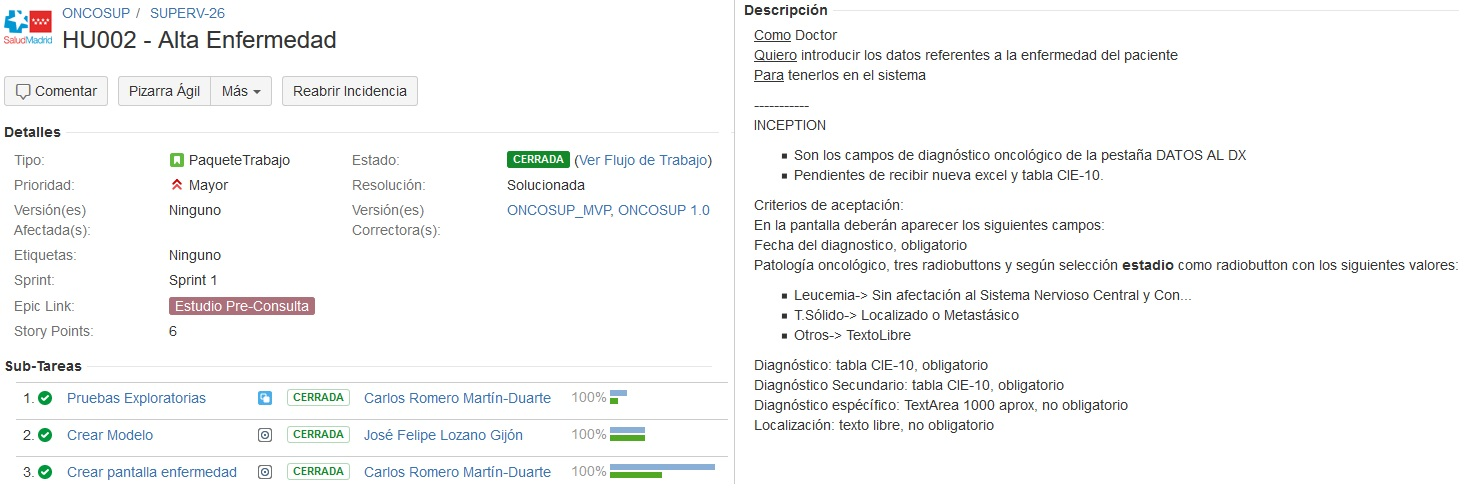
\includegraphics[width=1\textwidth]{HU002}
\caption{HU002 - Alta enfermedad}
\label{fig:HU002}
\end{center}
\end{figure}


\subsection{Desarrollo del sprint}
\label{subsec:S1-desarrollo}
Después de esta primera toma de contacto con los eventos de SCRUM, se empieza a valorar qué tipo de tareas podría comenzar a hacer la autora. Se decidió comenzar por tareas sencillas para, poco a poco, ir asignándole tareas más complejas como se verá en próximos sprints. 
Para el sprint 1 se le asignaron dos tareas: encargarse de la maquetación de las diferentes pantallas de la aplicación, y hacer el enlace entre un paciente y su diagnóstico, es decir asociar un diagnóstico existente en la base de datos a un paciente.

En cuanto a la primera tarea, la autora se encargó de averiguar cómo enlazar un archivo de estilos a un componente, y después generó unos estilos que en general y con algunas excepciones, se usarán en el futuro para todas las pantallas de la aplicación.

Para asociar un archivo de estilos a un componente es necesario ir a su archivo, y definir el nombre del archivo, tal y como se ve en el ejemplo del listado \ref{componentCSS}. Importante mencionar que es necesario que el archivo exista, a diferencia de en HTML que, si no se encuentra el archivo, simplemente no se cargan los estilos; en este caso la aplicación no compilaría.

\lstinputlisting[style=C, caption={Asociación de una hoja de estilos a un componente},label=componentCSS]{code/paciente-detail.java}

Respecto a los estilos, el listado \ref{estilos} muestra un ejemplo de cuáles son los estilos que se han creado para la web. La información del detalle de cada entidad se ha organizado de tal forma que los elementos relacionados están en un mismo "grupo", al contenedor de los elementos que forman parte de un grupo se le aplica la clase \emph{.block} y los atributos más importantes son \emph{display: flex} y \emph{flex-wrap:wrap}. Estos atributos le indican al navegador que si ese contenedor tiene más elementos de los que caben en la pantalla horizontalmente, debe pasarlos a la línea de abajo en cuánto uno no quepa, permitiendo añadir cuántos elementos queramos a un contenedor. Otra clase importante es \emph{.item}, que se le asigna a cada elemento dentro de un grupo (tanto título como valor). Con esta clase el navegador distribuye los elementos dentro de un grupo dándole un ancho del 25\% a cada uno, de esta forma tendremos 4 elementos en cada línea de un grupo. 

La clase \emph{.item-diagnostico} es un caso especial, el valor de este campo es un texto que puede ser de cierto tamaño, como no hay más elementos a su derecha, se ha decidido darle más anchura a ese elemento para que el texto se distribuya por toda la página aprovechando el espacio. Esto se repetirá en otras ocasiones en el futuro, debido a que, en diferentes pantallas, hay diferentes casos en los que es necesario redistribuir los elementos para aprovechar el espacio de forma más eficiente.

Desde este punto en adelante estos serán los estilos que se aplicarán a cada pantalla de detalle, con ligeras modificaciones como es la de la descripción del diagnóstico.

\lstinputlisting[style=C, caption={Estilos generales para páginas de detalle},label=estilos]{code/paciente.css}

En la parte final de los estilos aparecen las clases \emph{.half-block} y \emph{half-item} que son estilos específicos para los componentes de diálogo. Con \emph{justify-content: space-between} el navegador tratará de disponer los elementos de un contenedor separándolos tanto como pueda, para evitar que el navegador ponga un espacio demasiado grande, a cada elemento del bloque se le asigna un ancho de casi el 50\%, de tal forma que el navegador ponga solo un pequeño espacio entre los elementos. 

Las figuras \ref{fig:pacienteDetail} y \ref{fig:crearPaciente} muestran el resultado de estos estilos. Como se ha comentado en varias ocasiones JHipster genera una aplicación prácticamente funcional, así que la cantidad de estilos necesaria para maquetar los elementos no es elevada. El trabajo de la autora fue redistribuir los elementos para aumentar la usabilidad de la aplicación y hacer que fuese más \emph{user friendly}.

\begin{figure}[!h]
\begin{center}
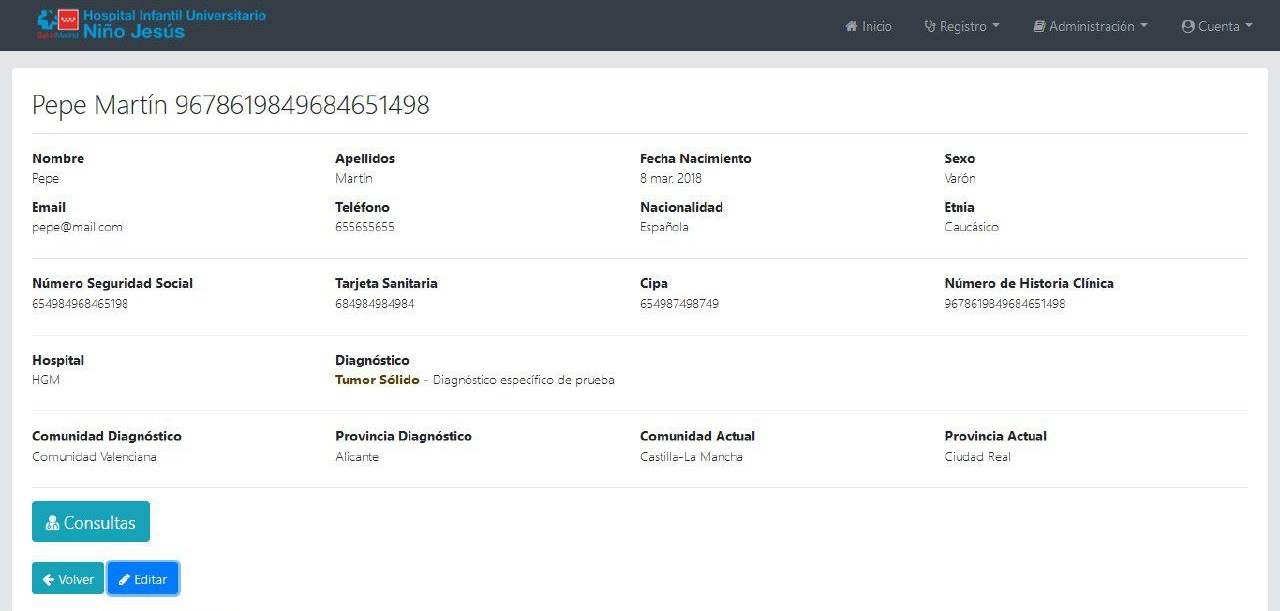
\includegraphics[width=1\textwidth]{paciente}
\caption{Detalle de un paciente}
\label{fig:pacienteDetail}
\end{center}
\end{figure}

\begin{figure}[!h]
\begin{center}
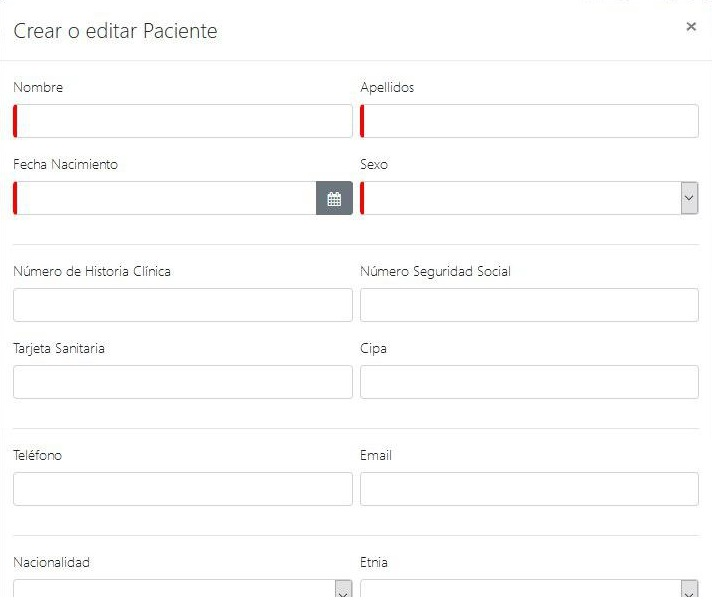
\includegraphics[width=1\textwidth]{crearPaciente}
\caption{Crear o editar un paciente}
\label{fig:crearPaciente}
\end{center}
\end{figure}

La segunda tarea de la que tuvo que encargarse la autora fue de enlazar un paciente con su diagnóstico a través de un \emph{id}. Esta tarea, que en un principio puede parecer sencilla de resolver con un sencillo script y añadiendo una variable en el paciente, con Angular5 no es tan sencillo. Si bien es cierto que Angular5 facilita muchas tareas, también es necesario aprender bien cómo funciona y habituarse a su uso.

Para realizar esta tarea no es necesario realizar cambios muy grandes, pero sí es necesario hacerlos en bastantes archivos. Para explicar esto se hará un recorrido desde el html del componente, hasta el guardado del \emph{id} en base de datos.

\lstinputlisting[style=HTML5, caption={Botón añadido al detalle del paciente},label=list:htmlPaciente]{code/paciente_detail.html}

En el html del detalle del paciente se añade un botón para la creación (Listado \ref{list:htmlPaciente}) y edición de un diagnóstico. A través del atributo \emph{routerlink} se indica qué elemento debe abrirse al hacer clic en el botón; en este caso \emph{diagnostico-new} abrirá el \emph{pop-up} para crear o editar el diagnóstico. A este \emph{routerlink} se le ha añadido el \emph{id} del paciente para, al mismo tiempo que se hace una consulta para crear el diagnóstico, hacer otra consulta que seleccione el paciente con dicho \emph{id} y le asigne el diagnóstico que acabamos de crear.

Este cambio no se puede hacer sin más, existe un archivo en el que se definen las distintas rutas a través de las que se puede abrir un componente, es necesario indicar este cambio también en ese archivo como muestra la figura \ref{list:diagnosticoRoute}, en la línea 5, dónde se ha añadido el \emph{id} del paciente a la ruta.
\\
\\
\lstinputlisting[style=C, caption={Código dónde se definen las rutas para el diálogo del diagnóstico},label=list:diagnosticoRoute]{code/diagnostico_route.ts}

Además, como último cambio en lo referente a las rutas y el paso de parámetros a través de éstas, necesitamos indicar al diálogo de edición del diagnóstico, que al abrir el \emph{pop-up} deberá pasarle como parámetro el \emph{id} que recibe en la ruta. En la parte superior del listado \ref{list:diagnosticoDialog} vemos que se hace una primera comprobación que verifica si se está recibiendo un \emph{id} (en este caso se trata del \emph{id} del diagnóstico), esta comprobación es para saber si debemos crear un diagnóstico nuevo o modificar uno ya existente. En ambos casos se ha añadido el parámetro \textbf{\textit{paciente\_id}} (líneas 7 y 9), con el fin de tener siempre identificado el paciente al que corresponde el diagnóstico.

\lstinputlisting[style=C, caption={Paso del \emph{id} al pop-up del diagnóstico},label=list:diagnosticoDialog]{code/diagnostico_dialog.component}

Tras esto se está enviando el \emph{id} del paciente en la ruta al abrir el diálogo de creación y edición de un diagnóstico, pero es necesario indicar que ahora tenemos una variable que contendrá el valor de este \emph{id}. 

Esto se soluciona en tres pasos, primero es necesario ir al archivo \emph{.model} correspondiente, en el que se especifican todos los atributos que va a tener una entidad, y añadir ahí la variable \textbf{\textit{paciente\_id}} que se va a recibir, de la forma en que se puede ver en la línea 17 de la figura \ref{list:diagnosticoModel} a continuación.
\\
\\
\\
\lstinputlisting[style=C, caption={Archivo .model del diagnóstico},label=list:diagnosticoModel]{code/diagnostico.model}

En el listado \ref{list:diagnosticoModel} se ha añadido un parámetro a la función \emph{open}, por tanto es necesario indicar en su declaración que recibirá este parámetro. La figura \ref{list:diagnosticoPopup} muestra en la línea 3 cómo se ha añadido esto a la declaración de la función. Además, en la parte en la que se guarda un diagnóstico al crearlo, se ha modificado de tal manera que ahora creamos el diagnóstico antes de guardarlo, así podemos asignarlo al paciente correspondiente antes de almacenar el diagnóstico creado, a diferencia de cómo se estaba guardando antes (comentario línea 8).
\\
\\
\lstinputlisting[style=C2, caption={Código del pop-up del diagnóstico},label=list:diagnosticoPopup]{code/diagnostico_popup.service}

En este punto sólo queda hacer la llamada para que el servidor efectúe las operaciones necesarias sobre la base de datos, para el paso de datos entre cliente y servidor, Angular5 utiliza un patrón denominado \emph{Data Transfer Object}(DTO) u objeto de transferencia de datos, que permite hacer de intermediario entre el cliente y el servidor, almacenando todos los cambios que se van realizando y permitiendo efectuar menos llamadas entre cliente y servidor. Así lo último que falta antes de poder guardar el \emph{id} del diagnóstico junto a su paciente es añadir el \emph{id} al DTO de diagnóstico. La figura \ref{list:diagnosticoDTO} muestra el código añadido a este archivo, que se corresponde con la declaración de la variable y sus métodos de consulta y modificación.

\lstinputlisting[style=C, caption={Código añadido al DTO de diagnóstico},label=list:diagnosticoDTO]{code/diagnosticoDTO.ts}

Tras todos los cambios explicados más arriba, ahora se puede ir al archivo \emph{DiagnosticoServiceImpl.java}, en el que se añaden, además de las importaciones pertinentes, las líneas 10, 11, 12 del listado \ref{list:diagnosticoServiceImpl}, que finalmente, tras guardar el diagnóstico, busca en la base de datos el paciente correspondiente al \emph{id} recibido, y le asigna el diagnóstico creado.

\lstinputlisting[style=C, caption={Asignación de un diagnóstico al paciente},label=list:diagnosticoServiceImpl]{code/diagnosticoServiceImpl.java}

Para el primer sprint se hizo un refinamiento en el \emph{Sprint planning}, pero para el resto de sprints lo habitual es aproximadamente a la mitad del sprint anterior se haga el refinamiento de las historias que podrían ser planeadas en el siguiente sprint, de esta manera en la segunda semana del primer sprint se hizo el refinamiento de las posibles historias que se planearían para el segundo. Esta rutina se repite a lo largo de todos los sprints.
 

\subsection{Sprint Review}
\label{subsec:S1-SR}
Finalizadas las dos semanas de duración del sprint, se hace la sesión de \emph{Sprint Review}. En esta reunión, a la que asiste todo el equipo, se hace un repaso por las historias que se habían planeado, para que tanto el equipo como el \emph{Product Owner} tengan fresco lo qué debería estar hecho a esta altura del sprint. Después se le explica al \emph{Product Owner} qué historias se han completado y cuáles no, y las razones por las que no ha sido posible completarlas, lo que se tendrá en cuenta en el siguiente \emph{Sprint Planning} para ajustar mejor la carga de trabajo que el equipo puede completar. Al finalizar el sprint 1 se completaron todas las historias de usuario a falta de la ``HU020A - Administrar Protocolos'' debido a que era una tarea muy grande, que, a pesar de tener múltiples subtareas completadas, al no estarlo todas, no se pudo cerrar.

Tras este breve repaso sobre las historias, se le enseña al \emph{Product Owner} el resultado del sprint. Como se explicaba en el \emph{Sprint Planning} al principio de la sección, estas reuniones se hacen a través de videoconferencia y compartiendo la pantalla de tal forma que todos puedan verla, de este modo se le puede hacer una demostración al \emph{Product Owner} de lo avanzado en la aplicación, haciendo un recorrido de cómo sería su uso, al menos hasta el punto en el que está el desarrollo. Afortunadamente, a pesar de no haber sido posible completar todas las historias planificadas, la \emph{Product Owner} queda muy contenta con lo que ha podido ver en este \emph{Sprint Review}, esta opinión es muy bien recibida por el equipo de desarrollo y se refleja en la \emph{Retrospectiva} a continuación.


\subsection{Retrospectiva}
\label{subsec:S1-Retrospectiva}

En la sesión de \emph{retrospectiva} el \emph{Scrum Master} selecciona una dinámica para que el equipo la lleve a cabo en esta sesión. En la pared se pondrán pósits, divididos en 3 categorías, lo que ha gustado, lo que no ha gustado y lo que se ha echado en falta. Cada miembro del equipo escribe en pósits y organiza según estas categorías sus sensaciones respecto al desarrollo del sprint. Cuando todos los miembros han anotado todo lo que querían, se explica el porqué de cada uno de sus pósits y se debate con el equipo la razón de haber puesto ese pósit en la pared. Esta sesión se trata de resaltar lo que se ha hecho bien y detectar los elementos que se pueden mejorar para enriquecer la experiencia del equipo en el desarrollo del proyecto.

En este sprint, algunas de las cosas se han destacado en la \emph{retrospectiva} han sido:
\begin{itemize}
	\item Cooperación con la \emph{Product Owner}. Según las experiencias del equipo en otros proyectos, no es habitual que el \emph{Product Owner}tenga una actitud tan positiva y facilite tanto el trabajo al equipo de desarrollo.
	\item Control de JHipster. A lo largo del sprint han ido surgiendo diferentes problemas que, poco a poco, el equipo de desarrollo ha ido resolviendo. Esto será de mucha utilidad a la hora de enfrentarse a problemas nuevos con la herramienta en el futuro ya que el equipo empieza a aprender cómo funciona JHipster.
	\item El cambio a Angular5. Aunque tanto para la autora como para los integrantes del equipo de desarrollo Angular era algo totalmente nuevo y difícil de aprender en un principio, valoran de forma muy positiva las posibilidades que ofrece.
	\item ``Tropezones positivos''. A pesar de haber tenido problemas y no haber sido capaces de terminar todas las historias del sprint, se valora mucho lo aprendido en estos ``tropezones'' de cara al futuro.
	\item El JDL (JHipster Domain Language) es una herramienta muy potente que permite definir tanto entidades como relaciones entre éstas, ahorrando mucho trabajo. En contraposición, un pequeño cambio en una entidad provoca que al volver a importar el JDL ésta se regenere por completo, habiendo perdido todos los cambios hechos. Este problema será algo con lo que tratar en cada sprint, ya que las diferentes entidades se van definiendo poco a poco y no tenemos toda la información de cada una de ellas desde el principio.
	\item El equipo proporcionado a la autora era antiguo y poco potente, lo que ha ralentizado su trabajo durante el sprint. 
	\item Historias demasiado grandes. Algunas historias tienen una carga de trabajo demasiado grande, como ha ocurrido con la historia ``HU020A - Administrar Protocolos''. \emph{JIRA} no permite cerrar una historia si no se han completado todas sus tareas, por lo que tuvo que quedarse sin cerrar a pesar de haber completado gran parte de ella.
\end{itemize}

De todo lo hablado durante la \emph{retrospectiva}, se acuerda tratar de conseguir un mejor equipo para la autora, y además se realiza un acuerdo de Trabajo; el equipo decide que todas aquellas historias de usuario que tengan más de diez puntos de historias serán divididas para simplificarlas en historias más pequeñas y fáciles de alcanzar.

Finalmente, a pesar de no haber conseguido acabar con todas las historias, tras el \emph{Sprint Review}  y la \emph{retrospectiva} el equipo cierra el sprint con buen sabor de boca y buenas sensaciones para el siguiente.
\clearpage
\section{Sprint 2}
\label{sec:sprint2}

Dos semanas después, tras la finalización del primer sprint, comienza el sprint 2, el día 19 de febrero y finaliza el día 2 de marzo.
 
\subsection{Sprint Planning}
\label{subsec:S2-SP}

Como se ha mencionado en varias ocasiones, la primera actividad que se realiza al comenzar un sprint es el \emph{Sprint Planning}. Durante el sprint anterior se realizó la sesión de refinamiento, en la que se concretaron los criterios de aceptación de las historias candidatas a ser planeadas para el segundo sprint. Con ese trabajo adelantado durante el primer sprint, esta reunión tiene menos duración que la del sprint 1.

Los miembros del equipo se reúnen, como es habitual, a través de videoconferencia con la \emph{Product Owner} para decidir qué historias son las que son capaces de aborda de cara a este sprint. Tras debatir cuáles son las historias que se tratarán de completar, y aplicar el acuerdo de trabajo acordado al final del sprint anterior, el \emph{Backlog} del sprint 2 se muestra en el cuadro \ref{historiasSprint2}.


\begin{table}[!h]
\centering
\caption{Historias planeadas Sprint 2}
\label{historiasSprint2}
\begin{tabular}{llr}
\rowcolor[HTML]{C0C0C0} 
\multicolumn{1}{c}{\cellcolor[HTML]{C0C0C0}Identificador} & \multicolumn{1}{c}{\cellcolor[HTML]{C0C0C0}Resumen} & \multicolumn{1}{c}{\cellcolor[HTML]{C0C0C0}Puntos historia} \\
HU020A                                                     & Administrar Protocolos                            & 12                                                          \\
\rowcolor[HTML]{EFEFEF} 
HU003                                                      & Alta Recaída              						   & 10                                                           \\
HU004A                                                     & Alta Tratamiento:Resumen Tratamiento              & 1                                                          
 \\
\rowcolor[HTML]{EFEFEF} 
HU004B                                                     & Alta Tratamiento:Quimioterapia                    & 3                                                          
\\
HU004C                                                     & Alta Tratamiento: Radioterapia                    & 2                                                          
\\
\rowcolor[HTML]{EFEFEF} 
HU004D                                                     & Alta Tratamiento: Cirugía                         & 2                                                          
\\
HU004E                                                     & Aldta Tratamiento: Trasplante                      & 10                                                          
\\
\rowcolor[HTML]{EFEFEF} 
HU004F                                                     & Alta Tratamiento: Otros tratamientos              & 2                                                          
\\
\end{tabular}
\end{table}


La historia \emph{Alta Tratamiento} tenía 20 puntos historia, bebido a que se acordó dividir las historias de más de 10 puntos en historias más pequeñas, se puede ver en el cuadro \ref{historiasSprint2}, cómo el equipo la ha dividido en 6 historias más pequeñas, siendo únicamente una de ellas superior a los 3 puntos. El equipo es consciente de que no debería haber quedado ninguna historia con tantos puntos como \emph{Alta tratamiento: Trasplante}, pero tras debatir cuál sería la mejor forma de hacer la división, se llegó a la conclusión de que esa historia no permitía dividirla en otras más pequeñas.

\begin{itemize}
\item HU002A - Administrar Protocolos. Es necesario poder crear protocolos, es decir, poder definir cómo se trata la dolencia de un paciente. Esta tarea quedó por terminar en el sprint anterior.
\item HU003 - Alta Recaída. Permite registrar una o más recaídas para un paciente.
\item HU004 Alta Tratamiento. Engloba todos los elementos que conforman un tratamiento y que es necesario poder crear antes de pasar la consulta con el paciente. Se divide en:
	\begin{itemize}
	\item HU004A - Alta Tratamiento: Resumen Tratamiento. Registrar un resumen de cuál es el tratamiento.
	\item HU004B - Alta Tratamiento: Quimioterapia. Dar de alta una quimioterapia a la que se le podrá asignar un fármaco de los que hayan sido creados previamente en la aplicación.
	\item HU004C - Alta tratamiento: Radioterapia. Registra la información relacionada con una radioterapia.
	\item HU004D - Alta tratamiento: Cirugía. Permite registrar una cirugía e indicar entre otros valores una amputación o no.
	\item HU004E - Alta tratamiento: Trasplante. Dar de alta un trasplante para un paciente.
	\item HU004A - Alta tratamiento: Otros tratamientos. Se trata de una opción que permite indicar si el paciente ha tenido algún tratamiento que no se corresponda con ninguno de los anteriores.
	\end{itemize}
\end{itemize}

Al igual que se vio en la sección \ref{subsec:S1-desarrollo}, también se especifican en \emph{JIRA} los criterios de aceptación para considerar que una tarea esté completada. En relación con los criterios de aceptación de una historia, cabe mencionar la \emph{Definición de hecho o Definition of done}, que se trata de una lista con ciertas condiciones que todas las historias deben cumplir para considerarlas completadas. El \emph{Definition of done} suele comenzar siendo una lista pequeña que va aumentando con el desarrollo del proyecto, de manera que a medida que el equipo detecta nuevas características que las historias deberían cumplir, las van añadiendo. En el sprint 2 las condiciones eran solo tres: las historias deben estar codificadas, probadas y maquetadas. 

\subsection{Desarrollo del sprint}
\label{subsec:S2-desarrollo}

Dado que la \emph{Product Owner} estuvo muy contenta con la poca maquetación que se le pudo mostrar en la Sprint Review del sprint 1 (ver sección \ref{subsec:S1-SR}), la autora siguió encargándose de ésta durante el resto de sprints. A parte de las tareas de maquetación, se le fueron dando a la autora tareas cada vez más complejas, aumentando su dificultad con cada sprint. 

Una de las nuevas tareas que se le encargó a la autora era investigar e implementar \emph{comboBox} dependientes; esto es, que en función del valor seleccionado en un \emph{comboBox} aparezcan unos valores u otros en otro \emph{comboBox}. Tras un poco de investigación sobre cómo permite Angular 5 hacer ésto la solución que se aplicó se explica a continuación. 

Primeramente en el código HTML del componente (listado \ref{comboComunidades}) es necesario añadir un par de cambios, en el primer \emph{comboBox} se añade una llamada al método ``onComunidadActual(paciente.comunidadActualId)'' cada vez que el valor seleccionado del combo cambia. En el segundo combo cambiamos la lista de la que se extraen los datos en el ''*ngFor'' a ``provinciaPaisActual''. 
\clearpage
\lstinputlisting[style=HTML5, caption={ComboBox dependientes},label=comboComunidades]{code/comboComunidades.ts}

Ahora solamente queda cambiar el contenido de la lista ``provinciaPaisActual'' en función del valor elegido. Para ello implementamos en el archivo \emph{ts} del componente la lógica del método ``onComunidadActual(paciente.conmunidadActualId)'' (listado \ref{onComunidadActualId}). El funcionamiento del método es sencillo, se inicializa la lista para que no contenga ningún valor, después se recorre la lista de provincias y se añaden a la lista únicamente las que tienen un \emph{id} que coincide con el de la comunidad seleccionada.

\lstinputlisting[style=C, caption={Implementación onComunidadActual(paciente.conmunidadActual)},label=onComunidadActualId]{code/onComunidadActual.ts}

La otra tarea que se le encargó a la autora fue que en el detalle del paciente apareciera el diagnóstico específico junto con el diagnóstico del paciente. El procedimiento para solucionar esto es similar a lo visto en el sprint 1. Primero se añade la variable y sus \emph{getter} y \emph{setter} en el archivo PacienteDTO.java (listado \ref{diagnosticoEspecificoDTO}).

\lstinputlisting[style=C, caption={Cambios necesarios en el DTO para mostrar el diagnóstico específico},label=diagnosticoEspecificoDTO]{code/dianosticoEspecificoDTO.ts}

Se mapea la variable en el \emph{PacienteMapper.java} para poder tener el valor en el DTO (listado \ref{diagnosticoEspecificoMapper}).

\lstinputlisting[style=C, caption={Línea añadida al PacienteMapper.java},label=diagnosticoEspecificoMapper]{code/diagnosticoEspecificoMapper.java}

Finalmente falta añadir este campo en el html como se puede ver en la línea 9 del listado \ref{diagnosticoEspecifico-detail}.

\lstinputlisting[style=HTML5, caption={adición de un span con el diagnóstico específico},label=diagnosticoEspecifico-detail]{code/diagnosticoEspecifico-detail.ts}

A pesar de que esta tarea fue sencilla, hubo algunos problemas para hacerla funcionar. Una vez realizados los cambios descritos más arriba, al compilar y levantar la aplicación no aparecía el diagnóstico específico en el detalle. Tras algo de investigación se detectó que el archivo \emph{PacienteMapperImpl.java}, que se genera con cada compilación, no se estaba sobrescribiendo, por lo que hubo que eliminarlo manualmente del directorio del proyecto para que se generase de nuevo al compilar la aplicación.



\subsection{Sprint Review}
\label{subsec:S2-SR}

Nuevamente tras las dos semanas de duración del sprint, todo el equipo se reúne para mostrar a la \emph{Product Owner} los avances conseguidos.

Al finalizar el sprint anterior hubo que añadir unos cambios a petición de la \emph{Product Owner}. Esto supuso un cambio de alcance en el segundo sprint que según \emph{JIRA} se correspondía con un 5\% del alcance del sprint 2.

La productividad del equipo aumenta también, algo que es habitual en los primeros sprints y que se suele estabilizar a partir del tercero. En el sprint 2 se consiguieron 34 puntos, 9 más que en el sprint anterior, en el que se completaron 25. A pesar de este aumento de velocidad del equipo de desarrollo en este sprint también queda una historia que no se ha podido completar, ``HU003 - Alta Recaída''.

A pesar de que, de nuevo hay una historia sin terminar, \emph{JIRA} ya comienza a proporcionar análisis y resultados que resultan interesantes respecto al avance del proyecto. La figura \ref{fig:prediccionSP2} muestra la predicción que ofrece la herramienta en lo referente a las fechas. Como se puede apreciar en la imagen, nos da tres fechas de finalización del proyecto, una fecha de finalización del proyecto, y además una optimista y una pesimista. Dado que el proyecto está estimado para seis sprints, se espera acabar el 5 de mayo, por lo que el aumento de velocidad del equipo parece acercarlos a esa fecha.

\begin{figure}[!h]
\begin{center}
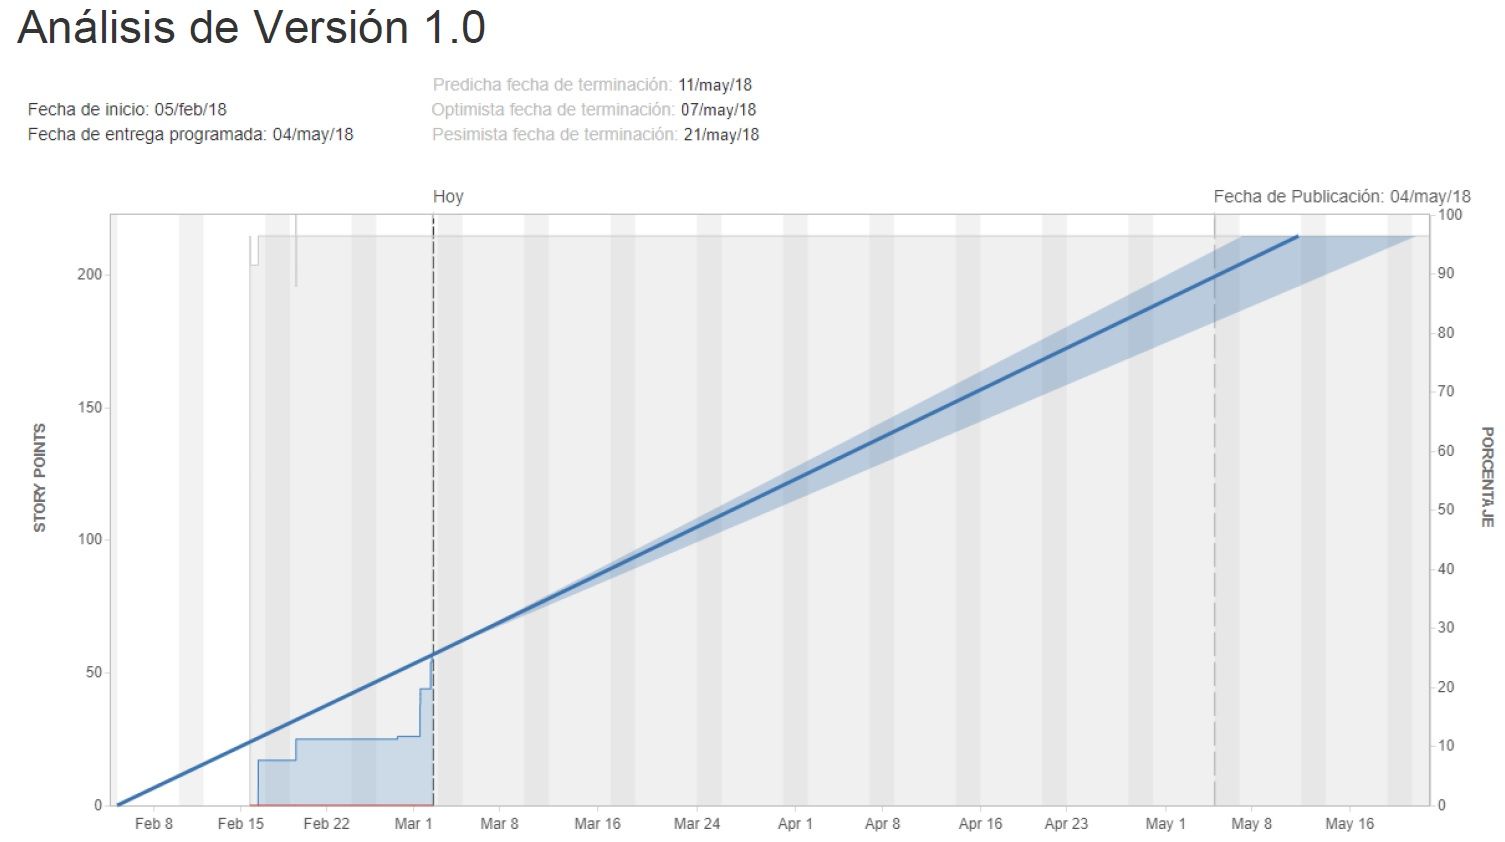
\includegraphics[width=1\textwidth]{prediccionSP2}
\caption{Predicción del avance del proyecto}
\label{fig:prediccionSP2}
\end{center}
\end{figure}


\subsection{Retrospectiva}
\label{subsec:S2-Retrospectiva}

En esta retrospectiva se trataron distintos temas. El más claro es que el equipo fue demasiado optimista a la hora de prever el trabajo que llevarían las diferentes historias relacionadas con el tratamiento, lo que supuso que el trabajo real necesario para completarlas fuese mayor que el estimado. En adelante el equipo será más cauteloso a la hora de hacer estas estimaciones para evitar que vuelvan a quedar historias sin terminar.

Además el equipo está muy contento con el desempeño de la \emph{Product Owner}, que valora el trabajo del equipo y da muy buena realimentación, lo que tiene un impacto positivo de cara al próximo sprint.

A pesar de no haber sido capaces de completar todo el alcance del sprint, el equipo está muy contento con la velocidad conseguida, y esperan ser capaces de aumentarla de cara al tercero.

La autora está cada vez más integrada en el equipo y los miembros valoran su aportación al proyecto. Consideran además, que su participación ha sido buena de cara a la \emph{Product Owner} que ha valorado positivamente ver pantallas maquetadas y con la información más clara.

Otro elemento que motiva al equipo es que cada vez se sienten más seguros con la arquitectura que proporciona JHipster y se sienten más cómodos trabajando con Angular5. Esto es importante de cara a los últimos sprints, en los que habrá que hacer más investigación para historias como las de crear el informe o exportar los datos a SPSS.

Por otro lado, el factor más negativo y que obliga al equipo a tener que rehacer trabajo cada sprint, son las limitaciones del JDL. Teniendo claros todos los elementos de la aplicación desde el principio y las diferentes relaciones entre ellos, el JDL es una forma muy sencilla y útil de generar gran parte del código. El problema que detecta el equipo es que, debido a la esencia de SCRUM, el proyecto debe hacerse en incrementos y pueden ir surgiendo cambios en el mismo, lo que obliga al equipo a generar un nuevo JDL al principio de cada sprint; esto supone volver a generar la aplicación y que cada entidad que haya sido modificada vea sobrescritos todos sus archivos.
\clearpage
\section{Sprint 3}
\label{sec:sprint3}

El sprint 3 da comienzo el día 5 de marzo y finaliza el día 16 de marzo.

\subsection{Sprint Planning}
\label{subsec:S3-SP}

En esta ocasión, al igual que en el sprint anterior, quedó una historia sin terminar, \emph{HU003 - Alta Recaída}, así que esta historia será planificada para este sprintu. El cuadro \ref{historiasSprint3}, a continuación, muestra las historias planificadas para este sprint.
\begin{table}[!h]
\centering
\caption{Historias planeadas Sprint 3}
\label{historiasSprint3}
\begin{tabular}{llr}
\rowcolor[HTML]{C0C0C0} 
\multicolumn{1}{c}{\cellcolor[HTML]{C0C0C0}Identificador} & \multicolumn{1}{c}{\cellcolor[HTML]{C0C0C0}Resumen} & \multicolumn{1}{c}{\cellcolor[HTML]{C0C0C0}Puntos historia} \\
HU003                                                      & Alta Recaída                            			& 10                                                          \\
\rowcolor[HTML]{EFEFEF} 
HU007                                                      & Alta Seguimiento Médico Actual				       	& 3                                                           \\
HU008                                                      & Alta Medicación Habitual                    		& 6                                                           \\
\rowcolor[HTML]{EFEFEF} 
HU018                                                      & Administrar Usuarios                    			& 13                                                          
\\
HU019                                                      & Auditoría                         					& 5                                                          
\\
\end{tabular}
\end{table}

\begin{itemize}
\item HU003 - Alta Recaída. Permite registrar una o más recaídas para un paciente. Esta tarea quedó por terminar en el sprint anterior.
\item HU007 - Alta Seguimiento Médico Actual. Da la posibilidad de dejar constancia en el registro de qué especialistas siguen de forma habitual a un paciente.
\item HU008 - Alta medicación Habitual. Se podrá relacionar ciertos fármacos con el tratamiento habitual de un paciente.
\item HU018 - Administrar Usuarios. Es necesario que la aplicación gestione diferentes roles para usuario, permitiendo acceder a diferentes funcionalidades dependiendo del rol que tenga asignado el usuario.
\item HU019 - Auditoría. Es necesario que quede un registro de las diferentes operaciones que se hagan en la aplicación.

\end{itemize}

\subsection{Desarrollo del sprint}
\label{subsec:S3-desarrollo}

En este sprint la autora se encargó de una historia completa, \emph{HU019 - Auditoría}. Para abordar esta historia se hicieron dos propuestas, crear una entidad Auditoría en la que se creará un nuevo registro por cada operación realizada, o, la que finalmente se escogió, aprovechar el módulo de Auditoría que incluye la propia aplicación. 

En el módulo de auditoría solamente se registran las autenticaciones, por tanto, era necesario añadir cada una de las operaciones que se realicen sobre pacientes con: la operación realizada, el usuario y la IP de origen de la operación. Para cada entidad dentro de paciente de la que sea necesario registrar la actividad se realizan las siguientes modificaciones. Se usa la entidad Quimioterapia como ejemplo de los pasos a seguir. 

En su archivo \emph{ServiceImpl.java} se importa el repositorio de la auditoría y se indica que la clase extiende del servicio Auditoría. Se crean unas constantes con la información que se mostrará para cada operación. Se añade al constructor y se inicializa. Por último, se indica que el método \emph{save} recibirá también una variable \emph{IP} y en función de si el guardado se trata de una actualización o una creación se crea la entrada de auditoría como creación o edición (\ref{quimioServiceImpl}. También se añade esto para el método delete.

\lstinputlisting[style=C, caption={Cambios en ServiceImpl para añadir auditoría},label=quimioServiceImpl]{code/quimioServiceImpl.java}

Ahora en el archivo Resource correspondiente, se importa el paquete HttpServletRequest para poder pasar la request a los métodos create, update y delete y extraer la ip desde la que se realiza la operación. El listado \ref{quimioResource} muestra ésto en el método \emph{deleteQuimioterapia}, el procedimiento es similar para el resto de métodos.

\lstinputlisting[style=C, caption={Cambios en Resource para añadir auditoría},label=quimioResource]{code/quimioResource.java}

Una vez añadidos estos cambios, si se accede a la auditoría desde la aplicación, se podrá ver un listado como el que se muestra en la figura \ref{fig:auditoria} con todas las operaciones realizadas.

\begin{figure}[!h]
\begin{center}
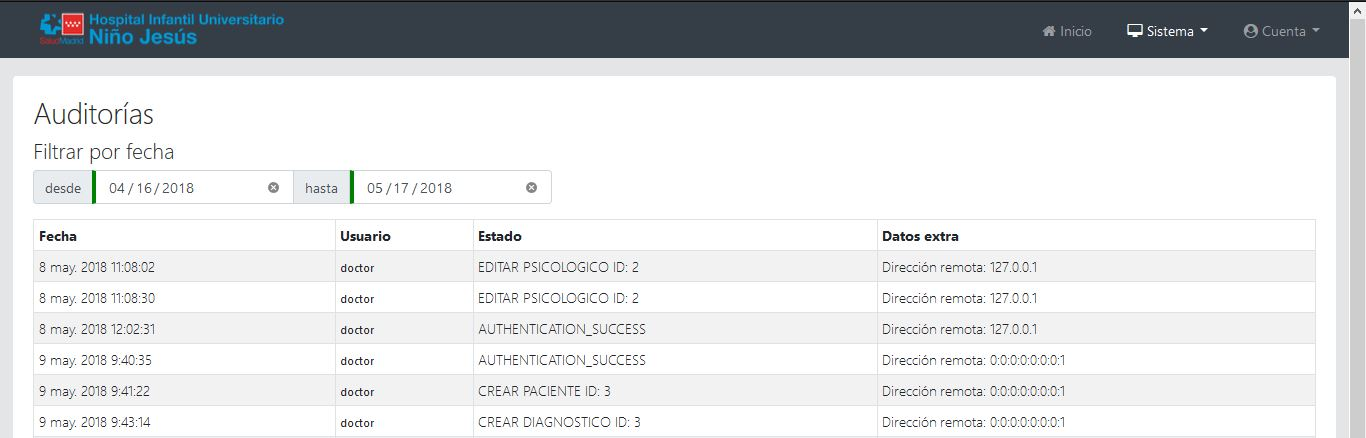
\includegraphics[width=1\textwidth]{auditoria}
\caption{Modulo de Auditoría}
\label{fig:auditoria}
\end{center}
\end{figure}

Por otra parte, la doctora solicitó poder filtrar y ordenar a los pacientes por año de diagnóstico, lo que implicaba añadir en el listado de pacientes una variable nueva con el año del diagnóstico, ya que los pacientes tienen un diagnóstico completo y no se almacena la fecha como un valor aparte. Para ello se añadió la nueva variable a la entidad paciente en el JDL, lo que genera automáticamente tanto la variable en el paciente y sus \emph{getter} y \emph{setter}.

Al crear o editar un diagnóstico se requiere que la variable que se acaba de crear se actualice con la fecha del diagnóstico. Esto se hace recuperando el paciente por su diagnóstico y asignándole el año del diagnóstico como se muestra en el listado \ref{annoDiagnosticoServiceImpl}.

\lstinputlisting[style=C, caption={Cambios en DiagnósticoServiceImpl para almacenar el año del diagnóstico en el paciente},label=annoDiagnosticoServiceImpl]{code/annoDiagnosticoServiceImpl.java}

Además, al resolver esta petición de la doctora, también se redujo el número de columnas mostradas en el listado de pacientes dejando únicamente las que la doctora consideraba relevantes para identificar pacientes de forma rápida, quedando como muestra la figura \ref{fig:listaPacientes}

\begin{figure}[!h]
\begin{center}
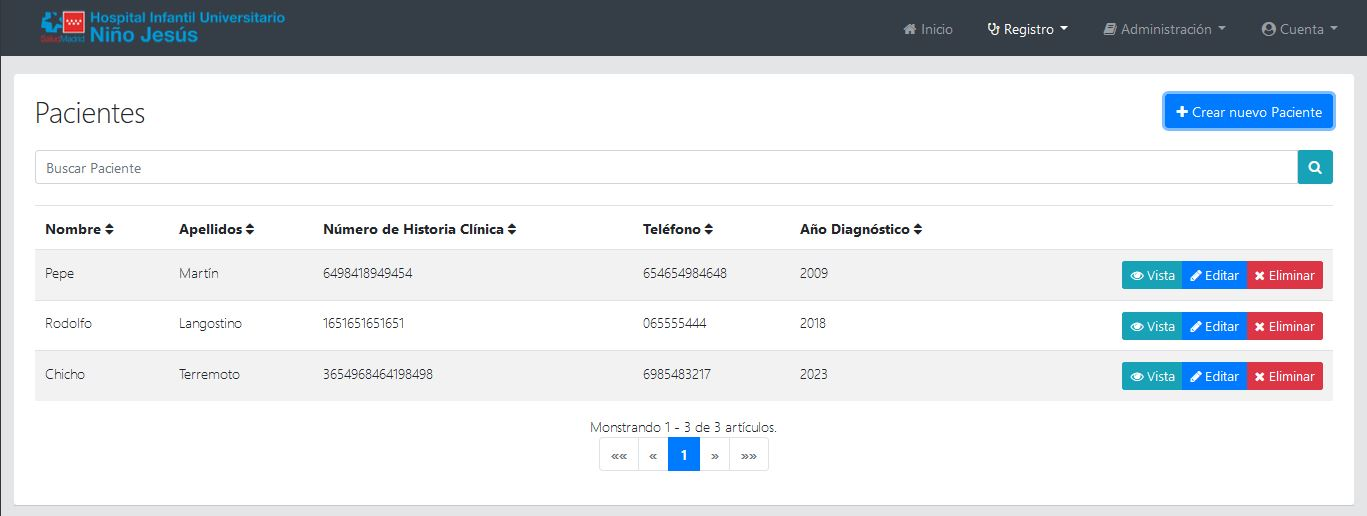
\includegraphics[width=1\textwidth]{listaPacientes}
\caption{Listado de pacientes una vez eliminados los campos innecesarios}
\label{fig:listaPacientes}
\end{center}
\end{figure}
\subsection{Sprint Review}
\label{subsec:S3-SR}

En este sprint el equipo finalmente consigue cumplir con todos los puntos planificados, aumentando la productividad en 3 puntos, con una velocidad de 37 puntos de historia. Además, se ha completado la versión MVP, que se correspondía con el estudio preconsulta. 

Otro punto que destacar de este sprint es que el equipo ha conseguido hacer una instalación de la aplicación en un entorno de pruebas, pudiendo comprobar así que no hay problemas con la instalación o con el funcionamiento de la aplicación lanzada directamente desde su war (Web Application Resource).

La retroalimentación de la \emph{Product Owner} acerca de los avances en la aplicación siguen siendo muy positivos, lo que mantiene al equipo motivado y comprometido.

Se comienzan a gestionar también algunos riesgos. Es necesario que se proporcione al equipo acceso a la red del hospital a través de VPN para poder hacer una instalación en el entorno de certificación y que la oncóloga pueda ir probando la aplicación para encontrar defectos. Este punto es importante, ya que, si no se detectan errores ahora, es posible que aparezcan al final del proyecto, cuando sea complicado gestionarlos.

Por otra parte, \emph{JIRA} a partir del tercer sprint ya empieza a darnos información y algunos gráficos interesantes. La figura \ref{fig:predivisiónSP3} muestra la estimación del avance por sprint que proporciona la herramienta. Según \emph{JIRA}, a este ritmo de trabajo, la duración del proyecto será de cinco sprints. A pesar de esta previsión el equipo cuenta con que es muy posible que aparezcan más cambios de alcance y se desarrollen seis sprints en total.

\begin{figure}[!h]
\begin{center}
\includegraphics[width=1\textwidth]{previsionSP3}
\caption{Previsión del avance del proyecto}
\label{fig:predivisiónSP3}
\end{center}
\end{figure}

\subsection{Retrospectiva}
\label{subsec:S3-Retrospectiva}

En este sprint el equipo ha completado el 100\% de los puntos planificados, y esto se refleja en la retrospectiva. Todo el equipo está muy satisfecho con la velocidad de este sprint, que les ha permitido, no solo completar todas las historias, sino también, probar la aplicación y buscar errores en ella. Esto último es muy importante debido a que, a causa del poco presupuesto, no hay equipo de testing en este proyecto; tener tiempo para comprobar que todo funciona como es debido, aunque sea solo haciendo pruebas manuales, ha sido muy útil para encontrar errores y pulir la aplicación.

Se destaca como punto positivo la capacidad que ha tenido el equipo para solucionar los problemas que han ido surgiendo, lo que refleja que es un equipo  y que es capaz de autogestionarse.

De nuevo sale a relucir lo contento que está todo el equipo con el desempeño de la \emph{Product Owner}, que este sprint ha estado más centrada que nunca.

Sin embargo, el JDL y sus limitaciones siguen saliendo como punto negativo del sprint.

Además, el equipo está descontento porque las historias crecen en alcance en los refinamientos, pero esto no queda reflejado después en \emph{JIRA}.

\section{Sprint 4}
\label{sec:sprint4}

El sprint 4 comienza el 19 de marzo, y finaliza el 6 de abril. Este sprint dura una semana más para compensar los días de vacaciones que tiene el equipo por Semana Santa.

\subsection{Sprint Planning}
\label{subsec:S4-SP}


Para este sprint, y tras hablar con la \emph{Product Owner} el equipo considera imprescindible dividir la historia \emph{HU009 - Alta Ítem} en tantas historias como ítems se puedan dar de alta en la aplicación. La estimación de estas historias se hace teniendo en cuenta que gran parte del código será reutilizado. Es por esto que la mayoría de los ítems tienen muy pocos puntos historia.

Prácticamente la totalidad de las historias planificadas (ver cuadro~\ref{historiasSprint4}), forman parte de la consulta y, a pesar de ser una cantidad considerable, una vez acabado el sprint, apenas se habrá completado la mitad de la funcionalidad de la consulta.

\begin{table}[!h]
\centering
\caption{Historias planeadas Sprint 4}
\label{historiasSprint4}
\begin{tabular}{llr}
\rowcolor[HTML]{C0C0C0} 
\multicolumn{1}{c}{\cellcolor[HTML]{C0C0C0}Identificador} & \multicolumn{1}{c}{\cellcolor[HTML]{C0C0C0}Resumen} & \multicolumn{1}{c}{\cellcolor[HTML]{C0C0C0}Puntos historia} \\
HU005                                                      & Alta Constantes									& 3                                                          \\
\rowcolor[HTML]{EFEFEF} 
HU006                                                      & Alta Exploración Física							& 6                                                           \\
HU009A                                                     & Alta Ítem Cardio									& 2                                                           \\
\rowcolor[HTML]{EFEFEF} 
HU009B                                                     & Alta Ítem Neumo									& 1                                                          
\\
HU009C                                                     & Alta Ítem Crecimiento								& 1                                                          
\\
\rowcolor[HTML]{EFEFEF} 
HU009D                                                     & Alta Ítem Peso										& 1
\\
HU009E                                                     & Alta Ítem Diabetes									& 1
\\
\rowcolor[HTML]{EFEFEF} 
HU009F                                                     & Alta Ítem Tiroides									& 1                                                          
\\
HU009G                                                     & Alta Ítem Maduración sexual						& 1                                                          
\\
\rowcolor[HTML]{EFEFEF} 
HU009H                                                     & Alta Ítem Nefrourológico							& 1
\\
HU009I                                                     & Alta Ítem Digestivo								& 1                                                          
\\
\rowcolor[HTML]{EFEFEF} 
HU009J                                                     & Alta Ítem Higado									& 1                                                          
\\
HU009K                                                     & Alta Ítem Piel										& 1                                                          
\\
\rowcolor[HTML]{EFEFEF} 
HU009L                                                     & Alta Ítem ORL										& 1
\\
HU009M                                                     & Alta Ítem Dientes-boca								& 1
\\
\rowcolor[HTML]{EFEFEF} 
HU009N                                                     & Alta Ítem Ojos										& 1
\\
HU009Ñ                                                     & Alta Ítem Hematológico								& 1
\\
\rowcolor[HTML]{EFEFEF} 
HU009O                                                     & Alta Ítem Vacunaciones								& 2
\\
HU009P                                                     & Alta Ítem Autoinmunidad							& 1
\\
\rowcolor[HTML]{EFEFEF} 
HU009Q                                                     & Alta Ítem Neurológico								& 1
\\
HU010                                                     & Alta Pruebas Complementarias que aporta			& 6
\\
\rowcolor[HTML]{EFEFEF} 
HU011                                                     & Alta Pruebas Complementarias solicitadas			& 6
\\
HU012                                                     & Alta Próxima Revisión								& 2
\\
\end{tabular}
\end{table}

\begin{itemize}
\item HU005 - Alta Constantes. Permite registrar valores constantes de un paciente como, por ejemplo: el peso, la altura, índice de masa corporal, etcétera.
\item HU006 - Alta Exploración física. Da la posibilidad de dejar constancia de cómo ha ido la exploración física que la oncóloga hace al paciente durante la consulta.
\item HU009 - Alta Ítem. Esta historia se divide en tantas historias como ítems hay en la aplicación. Debido a la gran cantidad de historias que han resultado de esta división, se comentan solamente las más relevantes:
	\begin{itemize}
	\item HU009A - Ítem Cardio. Permite registrar si el paciente tiene una complicación cardiológica. Esta historia tiene más puntos que el resto debido a que es la primera y, de la que se reutilizará la mayor parte del código.
	\item HU009(B-Q) excepto HU00O. Al igual que con el anterior, permiten registrar complicaciones sobre el ítem en cuestión además de otros campos relevantes. Estas historias tienen únicamente un punto debido a que se reutiliza el código generado para el primer ítem.
	\item HU009O - Ítem Vacunaciones. Este ítem tiene 2 puntos debido a que contiene más campos que los anteriores y más comprobaciones que los demás.
	\end{itemize}
\item HU010 - Alta Pruebas Complementarias que aporta. Permite al doctor registrar cualquier tipo de prueba que el paciente le aporte para el registro.
\item HU011 - Alta Pruebas Complementarias solicitadas. Si se solicitan pruebas por parte del oncólogo, aquí podrá registrar los resultados de estas.
\item HU012 - Alta Próxima Revisión. Permite reflejar la fecha de la próxima revisión del paciente, para que conste como una cita y aparezca en el informe, que se hará en próximos sprints.
\end{itemize}

\subsection{Desarrollo del sprint}
\label{subsec:S4-desarrollo}

En este sprint se animó a la autora a aprender cómo funciona el JDL añadiendo ella misma los ítems como entidades nuevas. 

Primeramente, se indican cuáles serán las nuevas entidades identificándolas con la palabra clave \emph{entity}. Se añaden los atributos que tendrá cada entidad como muestra el ejemplo del listado \ref{sprint4jdl} para el ítem cardio. Esta operación se realiza con cada uno de los ítems de la consulta.

También se usa la palabra clave \emph{relationship} para indicar las relaciones \emph{OneToOne} (ejemplo: una consulta tiene un ítem cardio) y \emph{OneToMany} (ejemplo: una consulta tiene una o varias pruebas aportadas)

\lstinputlisting[style=C, caption={Añadir nuevas entidades y sus relaciones en el JDL},label=sprint4jdl]{code/sprint4jdl.jh}

De la mano de la tarea anterior, se enseñó a la autora como crear historias y tareas en \emph{JIRA} para que ella misma pudiera encargarse de crearlas para cada uno de los ítems y comenzar a aprender más sobre la herramienta.

La creación de historias en \emph{JIRA} es sencilla. Estando en el espacio del proyecto, al hacer clic en la opción crear incidencia aparece una ventada de diálogo (figura \ref{fig:crearTareaJira}) en la que podremos definir, entre otros parámetros, el tipo de incidencia (en este caso ``story''), su nombre, el sprint al que pertenece, quién es el responsable, etcétera. Una vez creadas las historias, a través de un procedimiento similar, podemos acceder a cada una de ellas y añadirles las tareas, en las que además se añade la estimación de tiempo que requerirá llevarlas a cabo.

\begin{figure}[!h]
\begin{center}
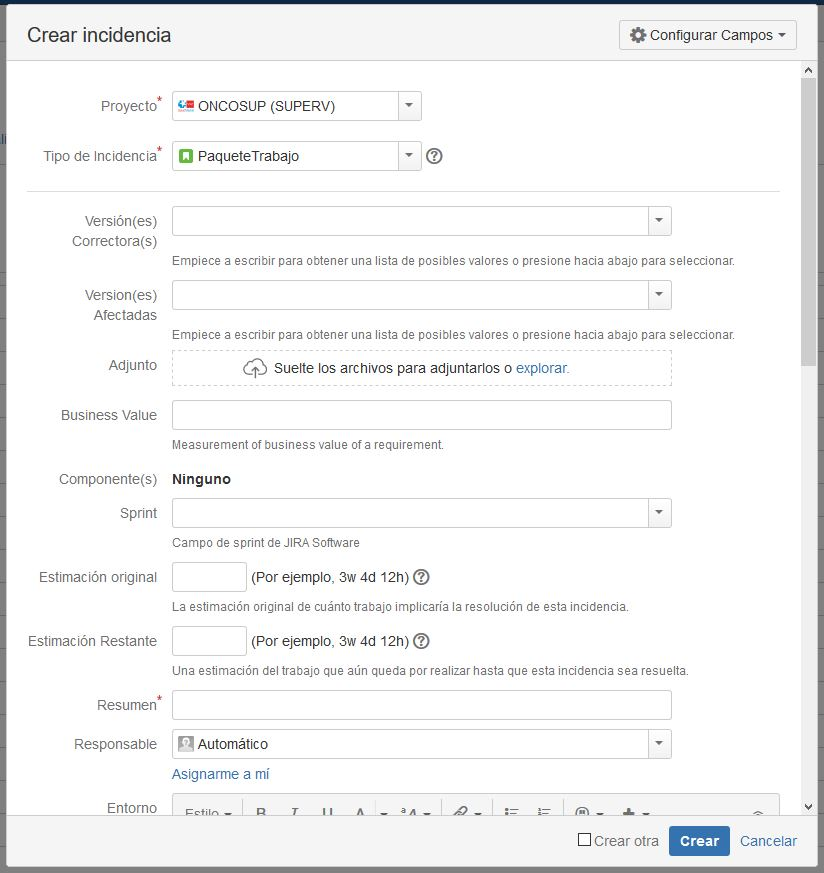
\includegraphics[width=1\textwidth]{crearTareaJira}
\caption{Creación de una incidencia en JIRA}
\label{fig:crearTareaJira}
\end{center}
\end{figure}

Debido a que en este sprint se terminó el trabajo estimado antes de lo previsto, se decidió añadir una historia más al trabajo del sprint, \emph{HU013 - Alta efecto tardío}. El trabajo de esta tarea se repartió entre los miembros del equipo, tocándole a la autora maquetar todas las pantallas y eliminar los botones de edición, creación y eliminación. La eliminación de los botones se debe a que un efecto tardío se crea solamente cuando en un ítem se marca la casilla de ``complicación'', siendo un elemento que no es posible crear de otra manera.

La maquetación se realizó de misma manera que se explicó en la sección \ref{subsec:S1-desarrollo} y respecto a los botones, simplemente se eliminó el código HTML correspondiente tanto de la pantalla del listado como de la pantalla de detalle.
\subsection{Sprint Review}
\label{subsec:S4-SR}

Al finalizar el sprint 4, el equipo no sólo ha completado todos los puntos planificados, sino que han sido capaces de aumentar el alcance del sprint añadiendo una historia más, \emph{HU013 - Alta efecto tardío} de 11 puntos historia. Los puntos totales completados en el sprint 4 son 54. La adición de esta historia en el sprint supone un aumento del 26\% del alcance, por lo que la productividad de este sprint ha sido muy buena.

Un buen gráfico que ofrece \emph{JIRA} para ver esto reflejado es el \emph{Burn Down Chart}, en el que se puede ver como el equipo va cerrando puntos y se van completando las distintas historias. Por gráficos como este es importante que las historias tengan un tamaño razonable, de manera que el equipo las pueda ir cerrando durante el desarrollo del sprint en lugar de todas de golpe al final. Esto facilita el seguimiento del desarrollo del sprint.

En la figura \ref{fig:burnDownChart} se puede observar que el equipo ha ido completando historias a buen ritmo durante todo el sprint, y que el día 2 de abril decidieron ampliar el alcance añadiendo una historia más. También se refleja en los días 3 y 5 de abril que se reabrieron dos historias para solucionar errores que se detectaron mientras se hacían pruebas ágiles en la aplicación.

\begin{figure}[!h]
\begin{center}
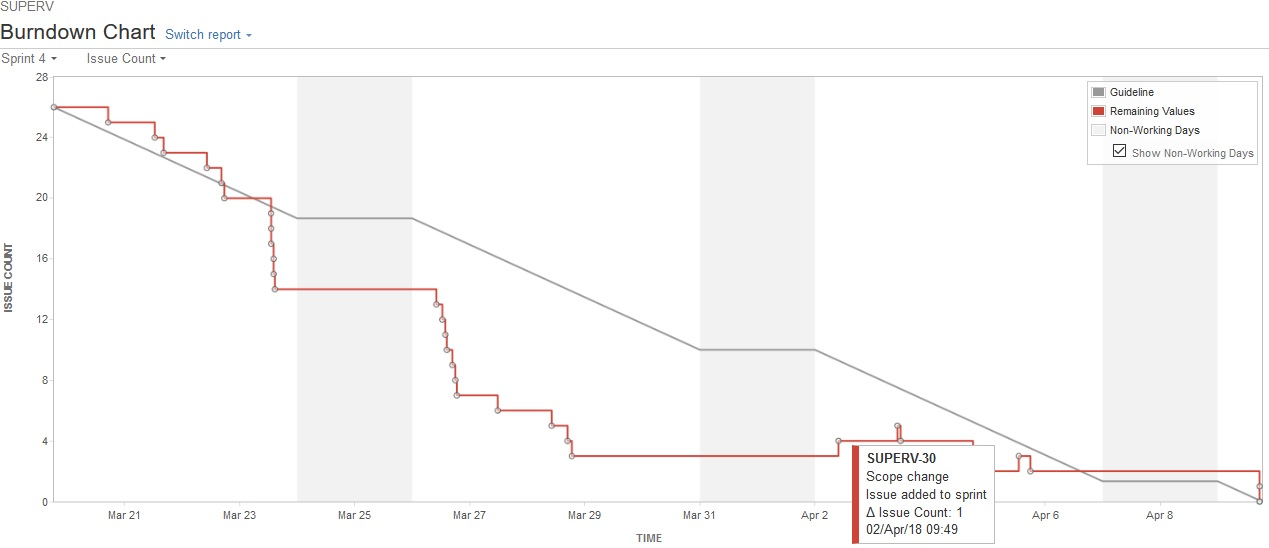
\includegraphics[width=1\textwidth]{burnDownChart}
\caption{Burn Down Chart del Sprint 4}
\label{fig:burnDownChart}
\end{center}
\end{figure}

En este punto del proyecto el equipo aún no ha sido capaz de solucionar el problema de acceso a través de VPN al entorno del hospital, por lo que se propone mitigar este riesgo realizando el próximo \emph{Sprint Review} en el propio Hospital, pudiendo así hacer la instalación \emph{in situ} y permitiendo así que la oncóloga pueda probar la aplicación y dar de alta defectos.

En la figura \ref{fig:prediccionSP4}, se muestra cómo la velocidad en este último sprint ha impactado positivamente en la fecha estimada de entrega, estando ahora mucho más acotada la fecha real prevista.

\begin{figure}[!h]
\begin{center}
\includegraphics[width=1\textwidth]{prediccionSP4}
\caption{Predicción del avance del proyecto}
\label{fig:prediccionSP4}
\end{center}
\end{figure}

Por otra parte, la figura \ref{fig:previsionSP4} muestra que \emph{JIRA} considera que el proyecto se seguirá completando en seis sprints. Desafortunadamente, el equipo considera que esta previsión no es fiable, ya que la reutilización de código en los ítems ha permitido alcanzar mucho más rápido y completar muchos más puntos de los esperado. Por tanto, prefieren ser prudentes y seguir contando con un sexto sprint para cerrar el proyecto.

\begin{figure}[!h]
\begin{center}
\includegraphics[width=1\textwidth]{previsionSP4}
\caption{Previsión de sprint restantes}
\label{fig:previsionSP4}
\end{center}
\end{figure}

\subsection{Retrospectiva}
\label{subsec:S4-Retrospectiva}

En este sprint el equipo en general está contento con la velocidad obtenida, pero son conscientes de que, debido a la reutilización de código en los ítems y a que debido a los días de vacaciones el sprint ha durado tres semanas, la velocidad no ha sido realista. De cualquier forma, están contentos con haber sido capaces de ampliar el alcance del sprint y reducir el trabajo restante para los dos próximos sprint.

El equipo sigue notando la falta de un tester y un plan de pruebas que les permita controlar que las diferentes funcionalidades de la aplicación funcionan correctamente. La velocidad de este sprint les ha permitido hacer ellos mismo pruebas exploratorias y corregir algunos defectos, pero les preocupa la alta probabilidad de que haya otros errores que puedan hacer que la aplicación no funcione como es debido.

Por otra parte, en el \emph{Sprint Review} la \emph{Product Owner} ha detectado que los efectos tardíos no se generan como ella quiso hacer entender al equipo, lo que implicará rehacer eso en cada ítem completado y asegurarse de que los nuevos se creen correctamente. El equipo detecta en este suceso un mal refinado de las historias del sprint que implica volver a codificar trabajo ya completado. La autora sugiere como medida para evitar que esto ocurra tratar de llevar bocetos o \emph{mockups} a los refinamientos para tratar de evitar confusión entre lo que el \emph{Product Owner} quiere transmitir y lo que el equipo entiende. Esto permitiría al \emph{Product Owner} hacerse una mejor idea de cómo será la aplicación viendo una simulación de cuál sería el funcionamiento de ésta y detectar errores antes de que se codifique. Todo el equipo considera que es una buena idea y se decide dar de alta una medida a tomar en \emph{JIRA} para que quede reflejado.

%\subsection{Análisis de la evolución de la aplicación}
%\label{subsec:S4-Analisis}



\section{Sprint 5}
\label{sec:sprint5}

La actividad correspondiente al sprint 5 comienza el día 9 de abril y acaba el día 20 del mismo mes.

\subsection{Sprint Planning}
\label{subsec:S5-SP}


En este sprint se planifican, entre otras, todos los ítems restantes a falta de los que no han sido refinados aún. Además la \emph{Product Owner} ha decidido dividir la historia del ítem ``musculoesquelético'' en dos distintas, quedando dos historias nuevas: \emph{HU009U1 - Alta Ítem Muscular} y \emph{HU009U2 - Alta Ítem Esquelético}.

\begin{table}[!h]
\centering
\caption{Historias planeadas Sprint 5}
\label{historiasSprint5}
\begin{tabular}{llr}
\rowcolor[HTML]{C0C0C0} 
\multicolumn{1}{c}{\cellcolor[HTML]{C0C0C0}Identificador} & \multicolumn{1}{c}{\cellcolor[HTML]{C0C0C0}Resumen} & \multicolumn{1}{c}{\cellcolor[HTML]{C0C0C0}Puntos historia} \\
HU009R														& Alta Ítem Neuropsicológico									& 1                                                          \\
\rowcolor[HTML]{EFEFEF} 
HU009U1														& Alta Ítem Muscular											& 1                                                           \\
HU009U2														& Alta Ítem Esquelético											& 1                                                          \\
\rowcolor[HTML]{EFEFEF} 
HU009V														& Alta Ítem Capacidad Física									& 1                                                          
\\
HU009W														& Alta Ítem Sexualidad											& 1                                                          
\\
\rowcolor[HTML]{EFEFEF} 
HU009Y														& Alta Ítem Fertilidad											& 1
\\
HU014														& Alta Recomendaciones											& 3
\\
\rowcolor[HTML]{EFEFEF} 
HU015														& Visualizar Informe											& 11                                                          
\\
HU022														& Administrar Recomendaciones									& 6                                                          
\\
\rowcolor[HTML]{EFEFEF} 
HU026														& Eliminar Información del informe								& 10
\\
\end{tabular}
\end{table}

\begin{itemize}
\item HU009(R-Y) - Alta distintos Ítems. Al igual que se explicó en el sprint anterior (Sección \ref{subsec:S4-SP}) deben permitir dar de alta diferentes ítems. Aunque con pequeñas diferencias en cuanto a sus atributos, los ítems son muy similares y también habrá bastante reutilización de código.
\item HU014 - Alta Recomendaciones. Dará posibilidad de seleccionar una o varias recomendaciones de las ya creadas para asignarlas a un paciente en una consulta. Además, permitirá introducir una recomendación personalizada si es necesario.
\item HU015 - Visualizar Informe. Permitirá visualizar una vista previa del informe que se le entregará al paciente.
\item HU022 - Administrar Recomendaciones - El doctor podrá dar de alta diferentes recomendaciones para poder asignarlas más tarde a la consulta de un paciente.
\item HU026 - Eliminar Información del informe. El doctor podrá abrir un diálogo de edición que le permitirá eliminar o añadir la información que considere oportuna para el informe de un paciente.

\end{itemize}


\subsection{Desarrollo del sprint}
\label{subsec:S5-desarrollo}

En este sprint se aprovecha que la autora ha ido adquiriendo conocimientos suficientes para encargarle todos los ítems, de los que esta vez se encargará ella sola. Esto implica que tendrá que encargarse de añadir cada nuevo ítem al JDL, importarlo a la aplicación, y realizar todos los cambios necesarios; esto incluye, añadir todo lo relacionado con la auditoría, añadirlo a la consulta, añadir sus métodos de creación, edición y eliminación a ésta, y realizar además todos los ajustes necesarios en su \emph{detail} y su \emph{dialog}.

Debido a que algunas de estas tareas ya se han explicado en secciones anteriores, ésta se centrará en hablar de la maquetación de los diálogos. Aunque ya se habló algo sobre maquetación en la sección \ref{subsec:S1-desarrollo}, se tratará de explicar en detalle cómo se decidió organizar la información de los diálogos tratando de priorizar la usabilidad y la experiencia del usuario.

En primer lugar, la figura \ref{fig:capacidadFisicaAntes} muestra cómo se ve la ventana de diálogo tal y como la genera JHipster. A pesar de que JHipster genera una aplicación totalmente maquetada, se puede apreciar que hay algunas cosas que son muy mejorables. Los \emph{check box} están separados de su etiqueta, lo cual puede confundir al usuario. La cantidad de campos que aparecen es demasiada, esto además de poder abrumar la vista del usuario, obliga a tener que desplazar la pantalla para poder ver todos los campos.



Al maquetar estas pantallas se trató de simplificar la información y agruparla de forma que fuese más fácil de comprender e identificar para el usuario. Para ello, se aprovecharon los \emph{check box} para controlar qué información se mostraría en caso de marcarlos. En este ejemplo en concreto, los grupos son: complicación, tratamiento y deporte habitual; quedando el campo alteración como un \emph{check box} independiente. La manera en que se hace esto con Angular5 es haciendo uso de \emph{*ngIf} al que indicaremos que muestre los campos cuando su \emph{check box} correspondiente esté marcado como se aprecia en el listado \ref{capacidadFisica}.

\lstinputlisting[style=HTML5, caption={Control de campos que se muestran según el \emph{check box} marcado},label=capacidadFisica]{code/capacidadFisica.html}

\begin{figure}[!h]
\begin{center}
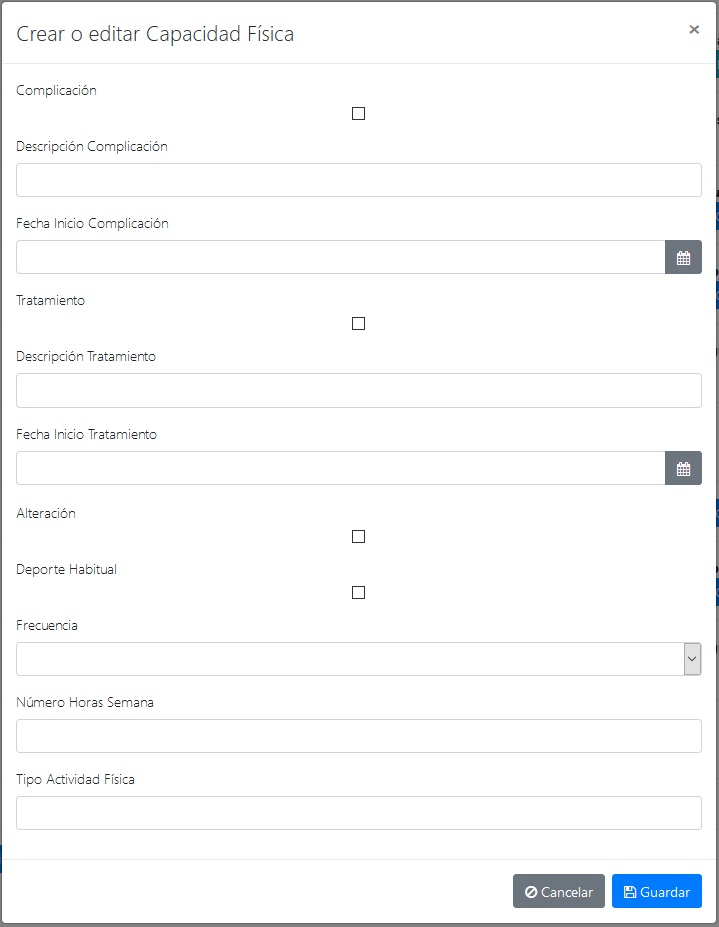
\includegraphics[width=1\textwidth]{capacidadFisicaAntes}
\caption{Diálogo de un ítem sin maquetar}
\label{fig:capacidadFisicaAntes}
\end{center}
\end{figure}

La apariencia del diálogo tras los cambios es la que muestra la figura \ref{fig:capacidadFisicaDespues}. Los campos que se muestran se han reducido a cuatro, que se desplegarán si el usuario marca alguno. Esta presentación es más legible para el usuario.

\begin{figure}[!h]
\begin{center}
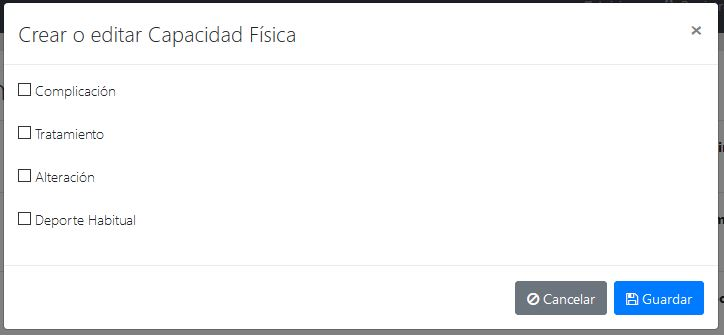
\includegraphics[width=1\textwidth]{capacidadFisicaDespues}
\caption{Diálogo de un ítem maquetado}
\label{fig:capacidadFisicaDespues}
\end{center}
\end{figure}

Cuando el usuario marque un \emph{check box} se desplegarán los campos como muestra la figura \ref{fig:capacidadFisicaDespuesDesplegado}, además, al desplegar un grupo de campos, se añade también un separador para que sea más claro dónde acaban. 

\begin{figure}[!h]
\begin{center}
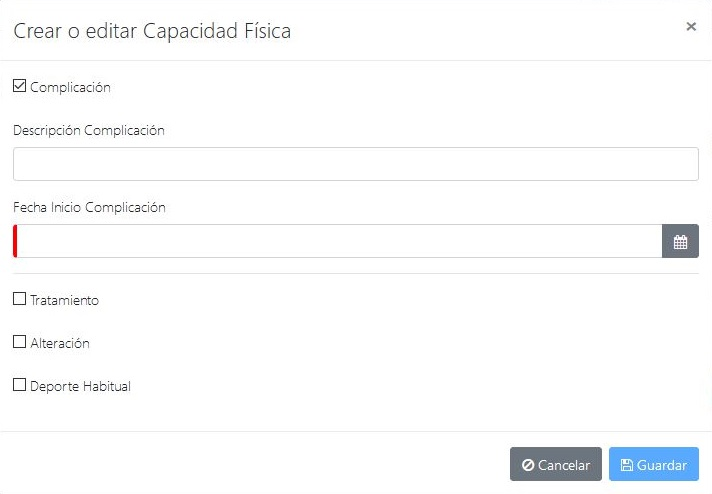
\includegraphics[width=1\textwidth]{capacidadFisicaDespuesDesplegado}
\caption{Diálogo de un item maquetado al desplegar un grupo de campos}
\label{fig:capacidadFisicaDespuesDesplegado}
\end{center}
\end{figure}

\subsection{Sprint Review}
\label{subsec:S5-SR}

El resultado de este sprint ha sido bueno debido de que el equipo fue precavido y no se dejó llevar por la alta velocidad obtenida en sprints anteriores, eligiendo menos historias debido a su mayor complejidad. Se ha completado toda la funcionalidad planeada para este sprint, pasando al siguiente sprint tan solo unas mejoras menores. Esto puede verse reflejado en la figura \ref{fig:burnDownChartSprint5}, dónde se aprecia que al acabar el sprint todavía quedaban algunos puntos por cerrar. Es interesante ver cómo, comparado con la figura mostrada en la sección \ref{subsec:S4-SR}, el equipo ha ido mucho más apurado en este sprint yendo por encima de la línea de progreso ideal que marca \emph{JIRA}.

\begin{figure}[!h]
\begin{center}
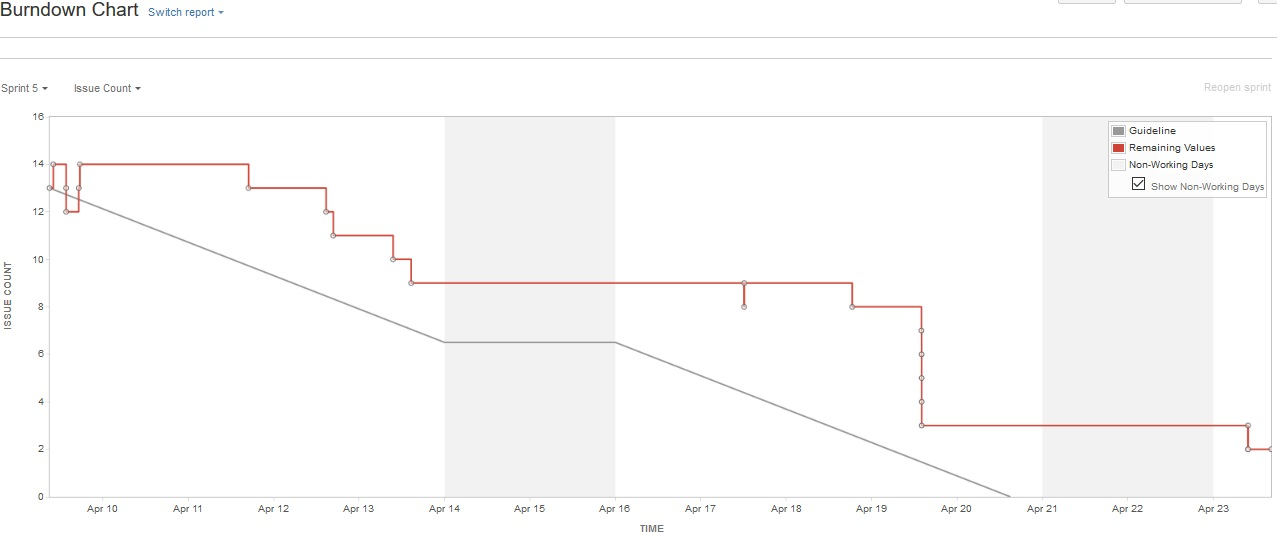
\includegraphics[width=1\textwidth]{burnDownChartSprint5}
\caption{Burn Down Chart. Sprint 5}
\label{fig:burnDownChartSprint5}
\end{center}
\end{figure}

Consultando la previsión de sprint restantes (figura \ref{fig:estimacionSprint5}) se puede ver que \emph{JIRA} estima un sprint más para completar todos los puntos de historia restantes, coincidiendo con las previsiones inciales del equipo.

\begin{figure}[!h]
\begin{center}
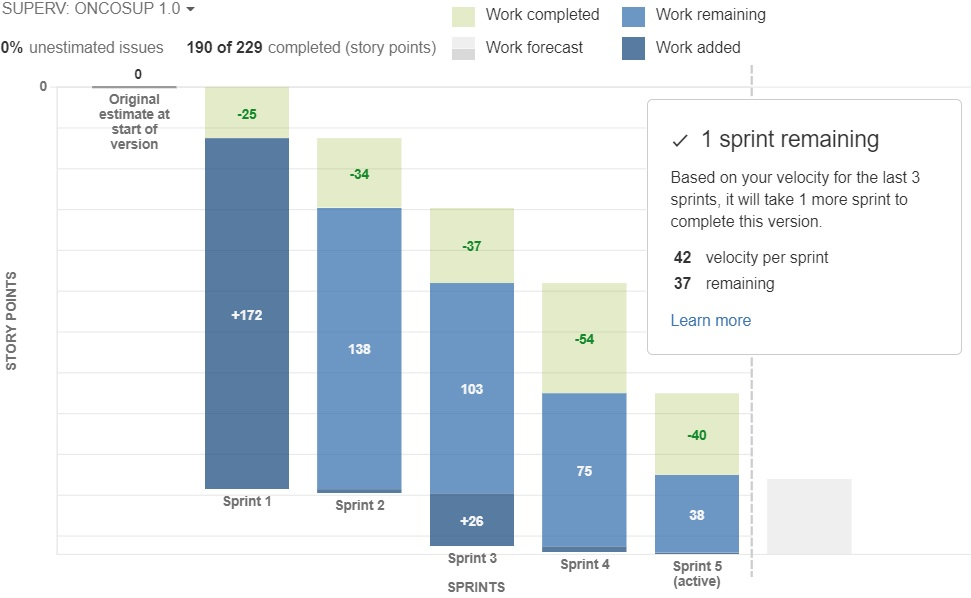
\includegraphics[width=1\textwidth]{estimacionSprint5}
\caption{Previsión de sprint restantes}
\label{fig:estimacionSprint5}
\end{center}
\end{figure}

\subsection{Retrospectiva}
\label{subsec:S5-Retrospectiva}

Nuevamente el equipo está muy contento con la reacción de la \emph{Product Owner} respecto a las soluciones que han aportado. Esto se debe a que, a la hora de presentar el informe, hubo un debate sobre cómo sería mejor hacerlo, y se llegó a la conclusión de que lo ideal es continuar con la misma tónica de toda la aplicación, el informe sería una entidad, su detalle serviría como previsualización y su diálogo serviría para añadir o quitar información. Tan solo sería necesario añadir un botón para la impresión, tarea que se acometerá en el próximo sprint.

Algo con lo que el equipo está muy contento es con el trabajo de Carlos, miembro del equipo que se ha encargado de preparar todo lo relacionado con la preparación de la instalación. Por otra parte, el equipo está satisfecho con haber podido realizar la instalación, a pesar de haberlo hecho de forma local en el ordenador de trabajo de la Dra. Herrero, ya que ahora será posible que la doctora prueba la aplicación y les reporte los errores de funcionamiento que detecte.

Además, el equipo se da cuenta de lo grande que es la aplicación y les agrada ver que a pesar de ser pocos miembros están siendo capaces de sacarla adelante.

Por otro lado, el equipo sigue preocupado por el hecho de que no haya un plan de pruebas, y los errores que la doctora notifique solo podrán ser corregidos durante el siguiente sprint. Por esta misma razón al equipo le gustaría que hubiera posibilidad de ampliar el presupuesto del proyecto para poder acabar la aplicación.

Finalmente, el Hospital aún no ha dado acceso a la VPN, y la instalación de versiones en el entorno de certificación del Hospital no va a poder hacerse.

%\subsection{Análisis de la evolución de la aplicación}
%\label{subsec:S5-Analisis}

\section{Sprint 6}
\label{sec:sprint6}

El sexto y último sprint comienza el día 23 de abril y acaba el día 4 de mayo.

\subsection{Sprint Planning}
\label{subsec:S6-SP}

En este último sprint se planean todas las historias de usuario restantes en el \emph{Product Backlog}. 

El cuadro \ref{historiasSprint6} muestra un total de puntos historia menor al que se podía ver en la figura \ref{fig:estimacionSprint5}, en la sección \ref{subsec:S5-SR}, esto se debe a que debido a que el equipo no considera que fuese capaz de completar toda la funcionalidad, se decidió eliminar una historia que la \emph{Product Owner} no consideraba vital para la aplicación.

\begin{table}[!h]
\centering
\caption{Historias planeadas Sprint 6}
\label{historiasSprint6}
\begin{tabular}{llr}
\rowcolor[HTML]{C0C0C0} 
\multicolumn{1}{c}{\cellcolor[HTML]{C0C0C0}Identificador} & \multicolumn{1}{c}{\cellcolor[HTML]{C0C0C0}Resumen} & \multicolumn{1}{c}{\cellcolor[HTML]{C0C0C0}Puntos historia} \\
HU000														& Login															& 7                                                          \\
\rowcolor[HTML]{EFEFEF} 
HU009S														& Alta Ítem Psicológico											& 3                                                           \\
HU009T														& Alta Ítem Social												& 3                                                          \\
\rowcolor[HTML]{EFEFEF} 
HU009U														& Alta Ítem Información											& 1                                                          
\\
HU009V														& Alta Ítem Segundo Tumor										& 1                                                          
\\
\rowcolor[HTML]{EFEFEF} 
HU017														& Imprimir Informe												& 7
\\
HU024														& Exportación a SPSS											& 5
\\
\rowcolor[HTML]{EFEFEF} 
HU025														& Filtro Exportación SPSS										& 3                                                          
\\
\end{tabular}
\end{table}


\begin{itemize}
\item HU000 - Login. Implementar una autenticación de usuarios que esté integrada con el LDAP del hospital.
\item HU009(S-V) - Alta distintos Ítems. Se debe permitir dar de alta los diferentes ítems. En este caso el ítem psicológico y el ítem social tienen tres puntos debido a que la complejidad de éstos es mayor que la del resto.
\item HU017 - Imprimir Informe. Permitirá imprimir el informe.
\item HU024 - Exportación a SPSS - Se trata de una opción que permite exportar toda la información de la base de datos de la aplicación a una hoja de cálculo que permitirá a la Dra. Herrero importar la información la herramienta SPSS.
\item HU025 - Filtro Exportación SPSS. Un filtro que permitirá elegir qué datos se desea exportar.
\end{itemize}

\subsection{Desarrollo del sprint}
\label{subsec:S6-desarrollo}

En este último sprint la autora tuvo que encargarse, además de los ítems restantes, de implementar la parte del informe referente a la impresión y algunos aspectos estéticos sobre la visualización e impresión de éste.

Para la impresión se decidió, por temas de tiempo, recurrir a la opción que al equipo le pareció más sencilla y que ofrecía un buen resultado: utilizar la herramienta de impresión del navegador. Esto permite que el navegador haga una impresión de la página usando los estilos que se han añadido en el \emph{.css}, con lo que sólo es necesario maquetar la pantalla una vez y no dos, una para la impresión y otra para la visualización. Hacer uso de esta herramienta es sencillo, al hacer clic en el botón imprimir que se ha añadido al final de la previsualización del informe, se hace una llamada al método \emph{print()} en el que se invocará la impresión del navegador (listado \ref{metodoPrint}).
\clearpage 
%El método \emph{print} realiza unas cuántas operaciones sencillasPREGUNTAR A JF PORQUE NO SE COMO EXPLICAR (listado \ref{metodoPrint})

\lstinputlisting[style=C, caption={Implementación del método print()},label=metodoPrint]{code/print.ts}

Lo único que se necesita es que no imprima ni los botones de la parte baja de la página, ni el \emph{headder} ni el \emph{footer}. Para ello, en el archivo \emph{.css} del informe (listado \ref{metodoPrintCss}), se hace uso de la etiqueta \emph{@media print} en la que se indica qué debe ocurrir cuando se va a imprimir la página. Se crea una clase que no se va a mostrar en la pantalla de impresión y que se aplicará al contenedor de los botones y además se indica que no se muestren tampoco ni el \emph{headder} ni el \emph{footer}. La etiqueta \emph{@media screen} sirve para crear estilos que se aplican solo cuando se está en la pantalla del navegador. En la pantalla se desea que se muestre el nombre del paciente, pero al imprimir tan solo se muestra un título.

\lstinputlisting[style=C, caption={Estilos específicos de la impresión},label=metodoPrintCss]{code/print.css}

El resultado de estos estilos se puede ver en las figuras a continuación. La figura \ref{fig:previsualizacionInforme} muestra cómo se ve la pantalla del informe antes de imprimir, mientras que la figura \ref{fig:impresionInforme} muestra el informe tal y como se verá al imprimirlo.

\begin{figure}[!h]
\begin{center}
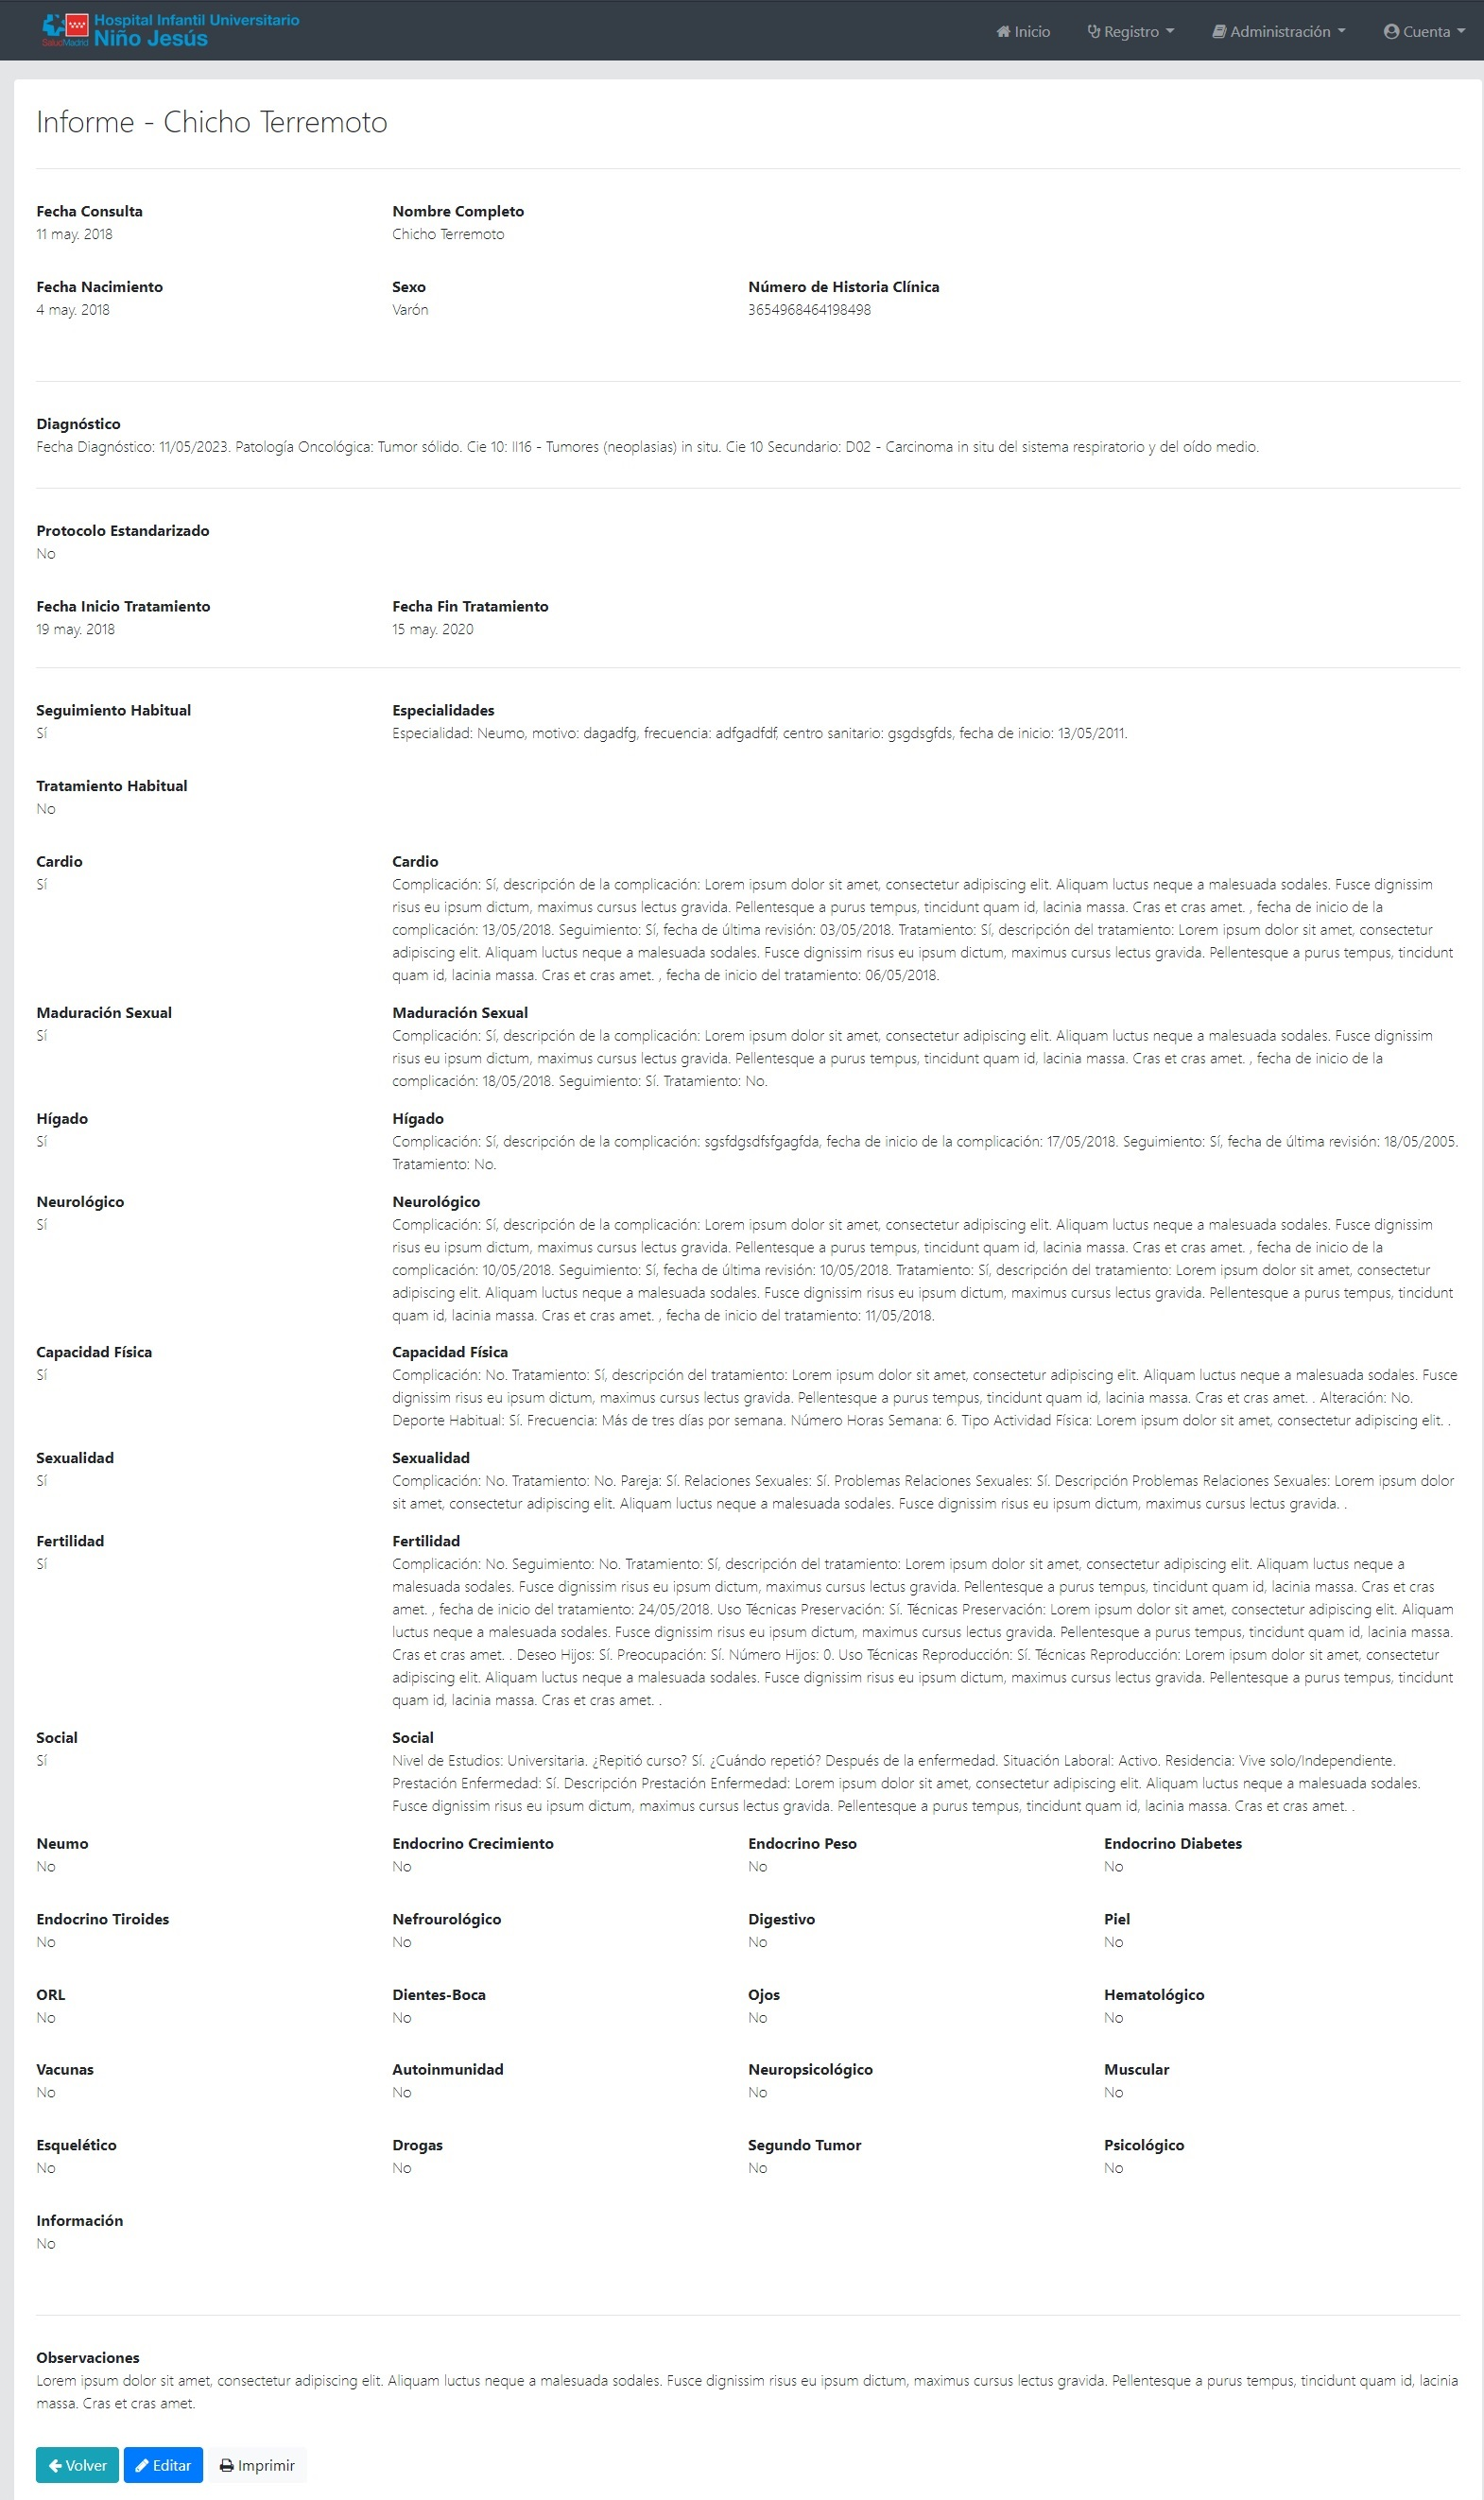
\includegraphics[height=\textheight]{previsualizacionInforme}
\caption{Previsualización del Informe}
\label{fig:previsualizacionInforme}
\end{center}
\end{figure}

\begin{figure}[!h]
\begin{center}
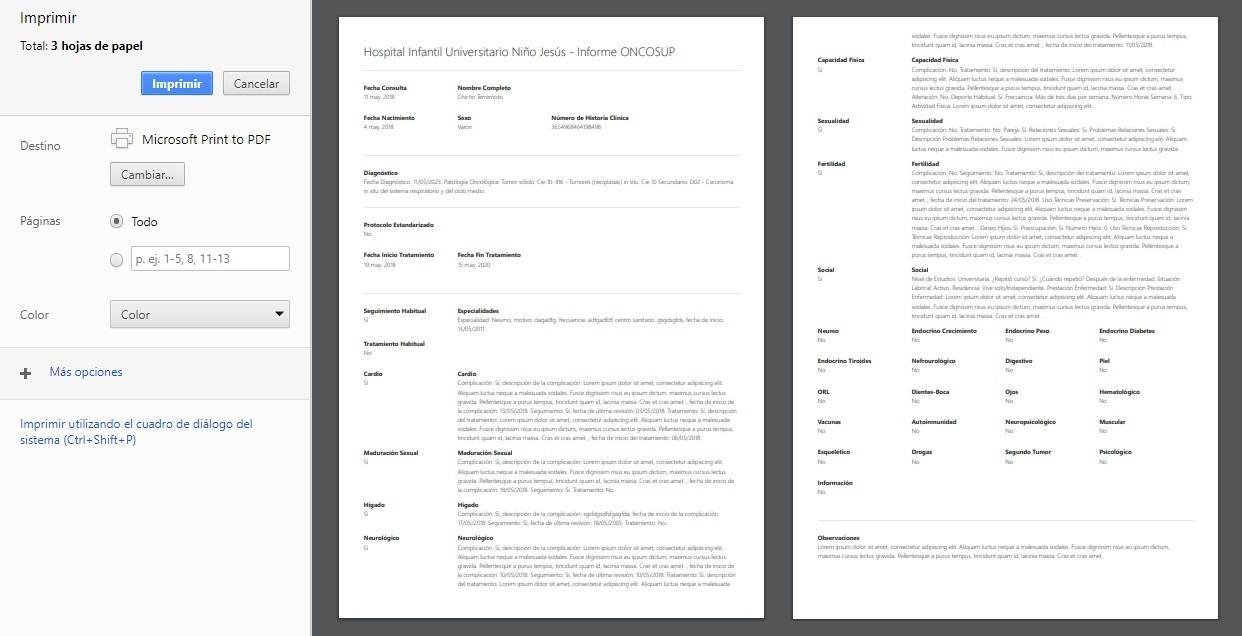
\includegraphics[width=\textheight, angle=-90]{impresionInforme}
\caption{Vista de impresión del informe}
\label{fig:impresionInforme}
\end{center}
\end{figure}
\clearpage
\subsection{Sprint Review}
\label{subsec:S6-SR}

En el sprint final del proyecto el equipo no ha podido completar todos los puntos planificados. El equipo no ha recibido la información necesaria para la integración de la aplicación con el LDAP, de manera que la historia \emph{HU000 - Login} ha quedado sin completar por causas ajenas al equipo.

Por otra parte, \emph{JIRA} indica que los cambios añadidos por la Dra. Herrero sobre algunas funcionalidades ya implementadas y la complejidad añadida a los ítems restantes han supuesto un incremento del alcance de un 14\%, alcance que sí se ha llegado a completar.

Si bien es cierto que la productividad del equipo ha sido menor que en los sprints anteriores, se debe a que al ser una versión final se ha dedicado más tiempo a corrección de defectos y por otra parte, el sprint 3 duró una semana más debido a las vacaciones. Esto, sumado a que una de las tareas planificadas ha sido imposible de completar, es la causa de este descenso en la productividad del equipo.

Algunos riesgos de los mencionados en la sección \ref{subsubsec:riesgos}, como son: \emph{R2 - Entornos no disponibles}, \emph{R3 - Acceso al hospital} y \emph{R4 - No se dispone de información sobre el acceso a LDAP} han acabado materializándose a pesar de los esfuerzos del equipo en mitigarlos, lo que ha impactado de forma negativa en el producto final.

Todo esto, unido a las restricciones económicas del proyecto ha provocado que el equipo no haya conseguido hacer entrega de la versión 1.0 tal y como estaba previsto, quedando alcance y funcionalidades que, para ser completadas, deberían ser acometidas en futuras fases o versiones de la aplicación.

\subsection{Retrospectiva}
\label{subsec:S6-Retrospectiva}

Con el desarrollo del proyecto ya acabado, el equipo se reúne para hacer la última retrospectiva. Esta retrospectiva no solo es sobre el sprint 6, sino que se analiza todo el proyecto y se trata de extraer un balance global.

Comenzando por lo positivo, todo el equipo está orgulloso de haber sido capaces de finalizar el proyecto a pesar del poco tiempo del que se disponía. Están muy contentos de que el primer proyecto hecho con JHipster haya salido tan bien, habiendo podido completar toda la funcionalidad en tan poco tiempo. Les gusta haber podido aprender tecnologías nuevas como Angular 5. Agradecen a la Dra. Herrero su participación como \emph{Product Owner} que, consideran, ha sido impecable.

En lo referente a las cosas que se deberían haber hecho mejor, les gustaría que hubiera habido mayor implicación por parte del departamento de informática del hospital, ya que ha supuesto la materialización de algunos de los riesgos detectados en la \emph{Inception}. Han echado en falta mayor apoyo institucional que diera visibilidad al proyecto. Las fuertes restricciones de presupuesto no han permitido dar ni siquiera un período de soporte para ONCOSUP.

Por último, el equipo expone que desearía respecto a este y otros proyectos basándose en lo vivido durante el desarrollo. Desearían que hubiera una segunda fase para ONCOSUP, para poder refinar la aplicación y añadir toda la funcionalidad que tuvo que descartarse en la \emph{Inception}. ONCOSUP ha obligado al equipo a valorar los recursos que tienen y creen que es algo que deberían tener en cuenta en próximos proyectos. El proyecto y la problemática que trataba ha sido una gran motivación para todos los miembros del equipo, y les gustaría que la motivación sea la misma en futuros proyectos. Esperan que ONCOSUP salga adelante, que cumpla el objetivo con el que fue concebida y no acabe olvidada en un cajón, sino que se expanda su uso y ayude a mejorar las vidas de los supervivientes y a salvar otras.

%\subsection{Análisis de la evolución de la aplicación}
%\label{subsec:S6-Analisis}